\chapter{Gradient-guided inpainting with a DDPM}
\label{chapter:gradpaint}

\chapterwithfigures{\nameref*{chapter:gradpaint}} \chapterwithtables{\nameref*{chapter:gradpaint}}

\ifthenelse{\boolean{skipGrad}}{\endinput}{}

\section{Introduction}

In the previous chapters, we tried two approaches to perform image editing to real images. In 
Chapter~\ref{chapter:magec}, we inverted a real image into a powerful pre-trained \ac{GAN} 
and thereafter applied known editing methods. However, although \ac{GAN} inversion can produce 
high-quality edits for in-domain images, fidelity to the real-image is time consuming and not guaranteed. 
In Chapter~\ref{chapter:flexit}, we  autoencoded a real image into a compact latent space and edited the resulting latent through 
the use of a pretrained \ac{CLIP} model and well-picked regularization terms. Although inversion in this case
is instantaneous, the editing relies on regularization terms rather than a generative prior, which may create poor edits.

In this chapter, we leverage another family of generative models, \ac{DDPM}, which can easily "invert" a real image 
into a \ac{DDPM} by simply noising it. Concretely, we aim to leverage a powerful \ac{DDPM} for the general 
task of inpainting. 
Inpainting consists in generating a missing part of a given image, given a binary mask 
indicating where the generation should take place. It is a fundamental task in computer
 vision, having obvious implications for image editing, image restoration, object 
 removal, and so on. We argue that if we have a robust unconditional 
inpainting method, then the extension to a more controlled generation (like stroke-guided editing~\citep{meng2022sdedit} or 
text-guided editing~\citep{nichol2021glide}) is also improved. The straightforward extension to real images, the strong generative power, 
and the iterative manipulation of spatial noise maps (which makes it easy to manipulate them with binary masks)  
of modern \ac{DDPM}s are our motivation to use pre-trained 
\ac{DDPM}s for this task. 


   There has been limited work in using pre-trained diffusion models for this task, and 
the typical approach~\citep{lugmayr2022repaint, meng2022sdedit, nichol2021glide} is to guide the generative 
model by replacing values of the intermediate noise map with noised pixels of the input 
image outside the inpainting mask, based on the hope that the denoising process inside 
the inpainting mask will progressively be biased towards image parts that blend 
naturally with the known surrounding context.
%iteratively combining a noisy masked ground-truth part with the masked generated part and denoising this constructed latent map with the pre-trained model. The intuition is that these combined noise maps, while corresponding to incoherent concepts at first, will gradually merge together into a harmonious image thanks to the denoising process \cite{meng2022sdedit}.
However, this strategy often produces unsatisfying results, which we believe is due to
 the diffusion model being strongly conditioned on the initial noise
  map~\citep{optimaltransport}, therefore having difficulties harmonizing the generation
   when the initial random latent map is too mismatched with the input image.


In this chapter, we quickly discuss the related work to contextualize our approach. 
Then, we introduce our strategy for guiding  pre-trained diffusion models
to better perform inpainting tasks. Our method, dubbed GradPaint, optimizes the
diffusion process by better harmonizing generated content inside the inpainting mask.
Specifically, we define a "harmonization" loss which depends on the prediction of the \ac{DDPM}
itself. Similar to classifier-guidance (see~\ref{subsection:classifier_guidance}), 
we use the gradient of this to  guide the generation at every single step of the denoising process towards a
more harmonized final image. We show extensive evaluation on various datasets, 
including  CelebA-HQ\citep{karras2018progressive}, FFHQ\citep{karra2019stylegan}, ImageNet\citep{deng2009imagenet},
Places2\citep{zhou2017places}, and COCO\citep{lin2014mscocodataset}. We discuss image diversity 
and generalization. Finally, we discuss some limitations and conclude. 

Our work is currently in submission:

\fullcite{grechka_gradpaint}


% Inpainting consists in generating a missing part of a given image, given a binary mask 
% indicating where the generation should take place. It is a fundamental task in computer
%  vision, having obvious implications for image editing, image restoration, object 
%  removal, and so on. Currently, state-of-the-art methods are generally based on 
%  Generative Adversarial Networks (GANs)~\citep{lama, zhao2021comodgan}, and consist 
%  in explicitly training a model to reconstruct an image using self-generated masks.
%   Although these methods often achieve reasonable results with standard metrics, 
%   visual results tend to have obvious, unrealistic artifacts. Moreover, training 
%   these models is accompanied with the difficulties of training instability inherent 
%   with GANs as well as limitations on the diversity of the dataset distribution. 

% Denoising diffusion probabilistic models (DDPMs) have recently gained massive attention,
%  achieving high-resolution, photo-realistic and diverse image generation 
% ~\citep{ramesh2022hierarchical, saharia2022photorealistic, rombach2022high, latentdiffusion2, nichol2021glide, dhariwal2021diffusion}. In 
%  terms of image generation, these models are on par or better than GANs even for 
%  constrained datasets like faces~\citep{rombach2022high}; and largely surpass them for 
%  diverse datasets like ImageNet~\citep{nichol2021glide, rombach2022high}. Furthermore, 
%  recent models trained on large-scale datasets 
% ~\citep{saharia2022photorealistic, ramesh2022hierarchical, nichol2021glide, gafni2022make, rombach2022high} have given rise to 
%  high-quality and flexible text-conditioned image generation, allowing users to 
%  generate astonishingly imaginative or artistic high-resolution images~\citep{artcomp}. 
%  It is thus highly enticing to be able to use these pretrained models directly for
%   downstream tasks, rather than re-training a new model from scratch. Here, we focus 
%   on the particular downstream task of inpainting.

% There has been limited work in using pre-trained diffusion models for this task, and 
% the typical approach~\citep{lugmayr2022repaint, meng2022sdedit, nichol2021glide} is to guide the generative 
% model by replacing values of the intermediate noise map with noised pixels of the input 
% image outside the inpainting mask, based on the hope that the denoising process inside 
% the inpainting mask will progressively be biased towards image parts that blend 
% naturally with the known surrounding context.
% %iteratively combining a noisy masked ground-truth part with the masked generated part and denoising this constructed latent map with the pre-trained model. The intuition is that these combined noise maps, while corresponding to incoherent concepts at first, will gradually merge together into a harmonious image thanks to the denoising process \cite{meng2022sdedit}.
% However, this strategy often produces unsatisfying results, which we believe is due to
%  the diffusion model being strongly conditioned on the initial noise
%   map~\citep{optimaltransport}, therefore having difficulties harmonizing the generation
%    when the initial random latent map is too mismatched with the input image.


% \matt{Je trouve que la suite et fin de l'intro est bien mais trop narative linéaire. A discuter mais peut etre essaie de rester un peu plus general pour ensuite rassembler en 2 bullets les main contrib algo/expe ou tu pourra pour chacune entrer plus dans le détail technique.}
% This key observation - that the initial latent map strongly conditions success or failure of inpainting - is the motivation for our work. We propose to address this problem with direct optimization of the latent map. 
% We add a step of gradient descent at every iteration of the denoising process to directly optimize the noise vector, with the explicit objective of harmonizing the generated part with the masked input image. We leverage the model's prediction of the denoised image at every time step, and calculate how well this denoised image matches our input image. This is measured using a masked L2 loss as well as an \emph{alignement loss} which measures smoothness at the frontier of the merged image parts. The combined loss is backpropaged directly into the diffusion model itself, and its gradient is used to improve the noise map at each step of the denoising process. We also study the best way to combine the masked generated part with the unmasked input part, and propose a general protocol for inpainting with diffusion models.


% In this paper, we propose a new strategy for guiding pre-trained diffusion models
% to better perform inpainting tasks. Our method, dubbed GradPaint, is optimizing the
%  diffusion process by better harmonizing generated content inside the inpainting mask.
%   This guides the generation at every single step of the denoising process towards a
%    more harmonized final image.  Our method aims to minimize or even eliminate all the 
%    artifacts and inconsistencies that generally persist on the images due to the masked
%     regions.
% We propose a training-free algorithm which is advantageous because (i) there is no need 
% to train a inpainting-specialized model whenever a new model is available, and (ii) 
% training-based methods must chose a mask distribution to train on, to which training-free
%  methods are agnostic. We perform an extensive evaluation on various datasets, 
%  including  CelebA-HQ\cite{karras2018progressive}, FFHQ\cite{karra2019stylegan}, ImageNet\cite{deng2009imagenet},
%   Places2\cite{zhou2017places}, and COCO\cite{lin2014mscocodataset}. 

% Our main contributions can be summed up as:

% \begin{itemize}
%     \item We propose a novel training-free algorithm to the denoising scheduling of 
%     diffusion models for the specific task of inpainting. We improve this inpainting
%      mechanism with the explicit goal of harmonizing the generated parts with the current context. 
%      Specifically, we use a custom \textit{alignment loss} and leverage the intrinsic nature of 
%      diffusion models through which we back-propagate and calculate a gradient to optimize our loss. 

%     \item We show that our method generalizes well to a variety of datasets and 
%     pre-trained models, including latent-diffusion models. We show that our method 
%     improves baseline methods and is even on par with equivalent models trained 
%     specifically for the task of inpainting.
% \end{itemize}

% We show that our simple modification to the denoising scheduling yields a massive improvement in both qualitative and quantitative results.  We validate our results on a variety of pre-trained conditional and unconditional models, including latent diffusion models. We improve baseline methods on various datasets, including CelebA-HQ\cite{celebahq}, FFHQ\cite{ffhq}, ImageNet\cite{imagenet}, Places\cite{zhou2017places}, and COCO\cite{cocodataset} and show that our method improves baseline methods and is even on par with equivalent models trained specifically for inpainting. 


\section{Related Work}

\minipar{Inpainting}

In~\ref{section:image_editing}, we discussed different editing methods. Particularly, inpainting can be 
seen as a particular case of image-to-image translation  in which the input image is a masked image with 
missing parts and the goal is to "fill in" the missing parts while leaving the rest of the image 
untouched. Historically, inpainting was aimed at recovering small corruption errors in images and 
was addressed with matching or ``borrowing" local color and texture around the masked
 region~\citep{poisson, patch_based}. Evaluation consisted in calculating a distance
  metric with respect to the unmasked image. More recently, generative models have 
  become capable of synthesizing realistic and diverse images, allowing the use of much
   larger masks when inpainting images. Generative models thus have more freedom 
   to ``imagine" a wide range of possibilities much different from the reference image,
    which is satisfactory (and oftentimes desired) so long as the resulting output looks
     realistic. 

In recent years, inpainting has been primarily addressed with training deep 
encoder-decoder convolutional networks from scratch, often using a 
GAN\citep{goodfellowgans} loss to encourage plausibility. Most recent work consists in 
improving the typical convolutional architecture in the encoder and/or decoder to better
 leverage structural or textural information from the surrounding regions 
 \cite{lama, hong2019deep, yu2020region, hukkelaas2020image, yang2020learning, zhu2021image, liu2018image, ma2022regionwise, zheng2022cm}. 
 \cite{li2020recurrent} proposes a progressive inpainting scheme which iteratively 
 fills in the mask by using surrounding information in the deep feature space.  
 \cite{xiong2019foreground, liao2020guidance} propose a framework to locate and 
 leverage semantic information.


% pre-trained models !??

In another line of work similar to ours, image completion is effectuated with the 
help of existing priors not specifically trained for the task.~\cite{ulyanov2018deep} 
trains a randomly initialized convolutional network to generate the input image, 
stopping training before overfitting occurs.~\cite{psp, zhao2021comodgan, glean} 
utilize powerful pre-trained decoders like StyleGAN2~\citep{karra2020stylegan2} and only train
 encoders to map the input image into the latent space of the decoder, which can produce
  more realistic results if the input image fits well to the distrubtion of the
   pre-trained decoder. 




%\matt{etoffer dire que c'est une etape des DDPM sampling modifié, qui compose avec la pred et le mask pour calculer un gradient dedie et le recombiner apres une interpolation pour calculer le next bruit ... Biensur la prediction direct n'est pas très bonne, recombinée avec l'image maskée cest mieux mais surtout ca permet de calculer des gradient sur tout xt utiles pour la prochaine reconstruction...}

\minipar{Diffusion models for downstream tasks}

As discussed in~\ref{sec:diffusion:models}, \ac{DDPM}s have become state of the art in 
image generation, including large-scale text-to-image generation as well as unconditional generation 
where \ac{GAN}s have typically excelled. They can also be conditioned
 on various input data: for the specific task of inpainting, the input image and mask 
 can be given as additional input to train a conditional diffusion model specialized on
  the inpainting task, as done in~\cite{saharia2022palette}.

However, due to the computational cost of training generative models, it is appealing 
to find adaptation algorithms for downstream tasks without fine-tuning, especially for
the task of inpainting which bears a lot of similarities with the unconditional 
generation task.~\cite{rombach2022high, nichol2021glide, song2021scorebased} propose to adapt
pre-trained diffusion models to inpainting by injecting a guiding mechanism in the 
generative process, a strategy which we build upon in this paper.~\cite{lugmayr2022repaint} also
proposes to take advantage of pre-trained diffusion models with cycles of denoising 
and renoising operations, which we found computationally very expensive. Finally, 
in a parallel line of work most similar to ours,~\cite{mcg} similarly propose to
guide the generation using the gradient of a ``manifold constraint", which they apply to 
various downstream tasks like inpainting, colorization, and sparse view CT reconstruction. 
While our method has similarities to~\cite{mcg}, we propose a guiding mechanism tailored to 
inpainting, outperforming their results.


\section{GradPaint Method}

%Given an input image $x_0$ masked out by a binary mask $m$, our goal is to generate a realistic image $x$ such that $x \odot (1-m) = x_0 \odot (1-m)$ and $x \odot m$ is generated.

% At a given timestep $t$ during the diffusion process, we use our pre-trained diffusion model to predict $\hat{x}_0$.

\subsection{Background: Inpainting-Guidance with Diffusion Models}\label{background}

Please refer to~\ref{subsec:diffusionmodels_framework} for the general framework of \ac{DDPM}s. 
In this subsection, we will build off the presented framework to describe the particular down-stream task of inpainting. 

% \ac{DDPM}s \cite{ho2020denoising} is a class of generative models trained with the following image denoising objective:

% \begin{equation}
%     \mathcal{L} = \displaystyle \mathbb{E}_{\x_0, t, \epsilon} \Vert \epsilon - \epsilon_\theta(\x_t, t) \Vert_2^2,
% \end{equation}

% where $\epsilon_\theta$ is a noise estimator network trained to predict the noise $\epsilon \sim \gaussian$  mixed with an 
% input image $\x_0$ in the following way: $\x_t = \sqrt{\alpha_t} \x_0 +  \sqrt{1 - \alpha_t} \epsilon$. This training is 
% performed for different values of the mixing coefficient $\alpha_t$, monotonically decreasing from $\alpha_0 = 1$ 
% (no noise) to $\alpha_T \simeq 0$ (almost pure noise) for a large integer $T$.

% At inference time, a new sample from the training distribution can be obtained by starting from random Gaussian 
% noise $\mathbf{x}_T \sim \mathcal{N}(\mathbf{0}, \mathbf{I})$, and iteratively refining it with the noise estimator 
% network with the following equations, called \textit{DDPM sampling equations} \cite{ho2020denoising}:

% $x$ and $\x$
% \begin{align*}
% \hat{\x}_0 & = \frac{1}{\sqrt{\alpha_t}}(\x_t - \sqrt{1 - \alpha_t} \cdot \epsilon_\theta(\x_t, t)), \numberthis \label{eq:ddpm1}\\
% %\x_{t-1} & = \sqrt{\alpha_{t-1}} \hat{\x}_0 + \sqrt{1 - \alpha_{t-1} - \sigma_t^2} \cdot \x_t + \sigma_t \boldsymbol{z}, \numberthis
% \x_{t-1} & = \frac{(\alpha_{t-1}-\alpha_t) \sqrt{\alpha_{t-1}}}{\alpha_{t-1}(1 - \alpha_t)} \hat{\x}_0 + \frac{(1-\alpha_{t-1})\sqrt{\alpha_t}}{(1 - \alpha_t)\sqrt{\alpha_{t-1}}} \x_t + \sigma \boldsymbol{z},
% \end{align*}
% where $t$ goes from $T$ to $0$, 
% $\sigma_t$ is a variance parameter, and $z \sim \gaussian$.

As presented in~\ref{subsec:diffusionmodels_framework}, the \emph{DDPM sampling equations} are as follows:

\begin{align*}
  \hat{\x}_0 &= \frac{1}{\sqrt{\alpha_t}}(\x_t - \sqrt{1 - \alpha_t} \cdot \epsilon_\theta(\x_t, t)), \numberthis \label{eq:ddpm0}\\
  \x_{t-1} &= \frac{(\alpha_{t-1}-\alpha_t) \sqrt{\alpha_{t-1}}}{\alpha_{t-1}(1 - \alpha_t)} \hat{\x}_0 + \frac{(1-\alpha_{t-1})\sqrt{\alpha_t}}{(1 - \alpha_t)\sqrt{\alpha_{t-1}}} \x_t + \sigma_t \z, \numberthis \label{eq:ddpm1}
\end{align*}


This iterative refinement can be ``guided" to impose constraints on the generated sample $\x_0$. In the case of inpainting, 
the aim is that the generated image exactly matches the input image outside a given inpainting region. The variable $\hat{\x}_0$, 
available at each timestep, represents the model's current estimation of what the denoised image will look at the end. 
For instance,~\cite{nichol2021glide} applies a maskwise correction on $\hat{\x}_0$ at each timestep:
\begin{equation}
\hat{\x}_0' = M \odot \hat{\x}_0 + (1 - M) \odot I,
\end{equation}
where $I$ is the input image and $M$ is a binary image mask equal to 1 in the image regions that must be inpainted, 0 otherwise. 
The update rule for $\x_{t-1}$ is then adapted to use $\hat{\x}_0'$ instead of $\hat{\x}_0$ in~\autoref{eq:ddpm1}. This correction 
progressively biases the diffusion model to exactly match $I$ outside the inpainting mask $M$. In the remaining of the paper, 
we refer to this method as \textit{combine-image} since it combines the images $\hat{\x}_0$ and $I$ before interpolating with $\x_t$.

Alternatively,~\cite{song2021scorebased, rombach2022high, lugmayr2022repaint} propose to directly correct $\x_{t-1}$ by replacing 
regions outside $M$ with the noised regions of the input image $I$:
\begin{equation}
\x_{t-1}' = M \odot \x_{t-1} + (1-M) \odot (\sqrt{\alpha_{t-1}} I +  \sqrt{1 - \alpha_{t-1}} \epsilon),
\end{equation}
where $\epsilon \sim \gaussian$ is resampled at each step. This $\x_{t-1}'$ is then used as input for the next denoising step 
instead of $\x_{t-1}$. We will refer to this method as \textit{combine-noisy} since it combines $\x_{t-1}$ inside the mask with 
ground truth (noised) pixel values outside the mask.


\subsection{GradPaint framework}

\begin{figure*}[h]
  \centering
    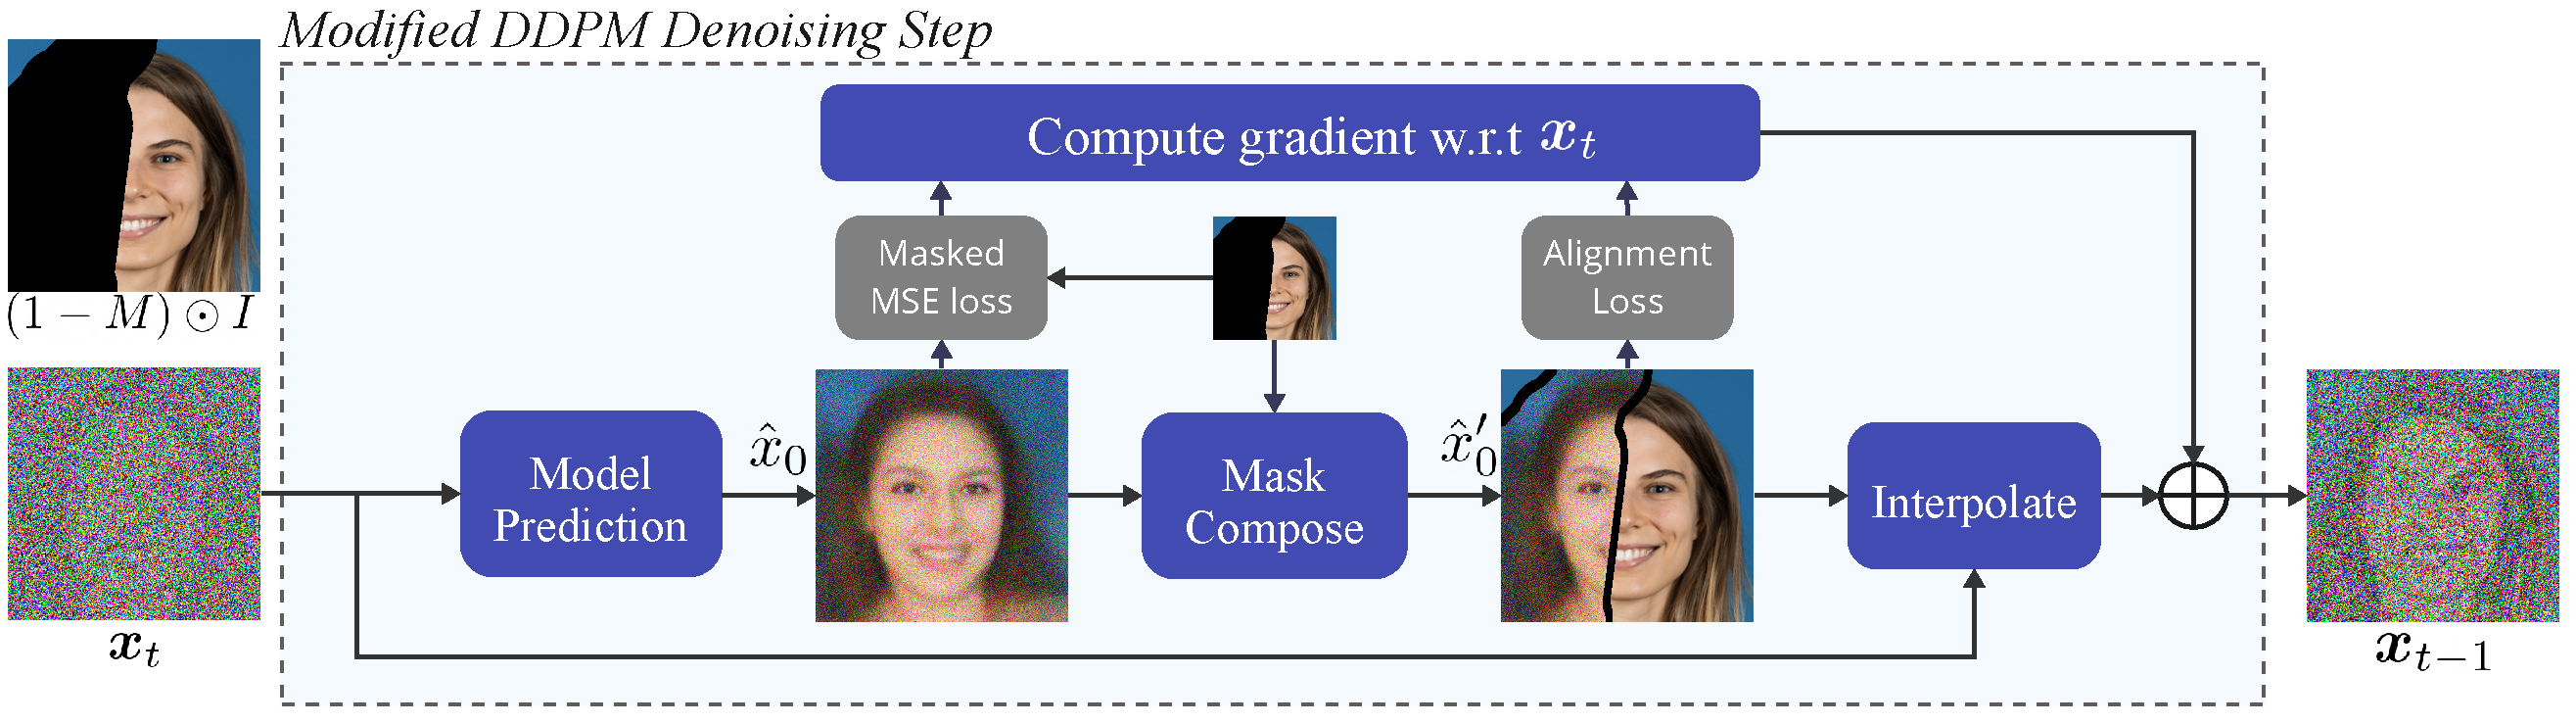
\includegraphics[width=\textwidth]{images/gradpaint/method.pdf}
    \caption{GradPaint method overview. We propose to modify one step of the DDPM denoising process with a gradient descent update on $x_t$ to better match the masked input image, in turn producing a better matched noise map $x_{t-1}$ for the next step. This improvement in the DDPM noise prediction thus allows for better fitting intermediate noise map predictions $x_t$ earlier in the DDPM denoising process, which ultimately produces a successful final inpainted image $x_0$.}
    \label{fig:method}
\end{figure*}


Our strategy is built upon the \textit{combine-image} zero-shot inpainting method presented in \S\ref{background}.
 Our key observation is that the most asthetically-pleasing inpainting results are obtained when the 
 collage $M \odot \hat{\x}_0 + (1-M) \odot I$ is coherent right from the beginning of the generation process.
  When this is not the case, there is a mismatch between the model's estimation in the inpainting region and 
  the known regions of input image $I$. This mismatch is generally present from the beginning and is not fully 
  corrected during the denoising generation process. 
%\matt{FAIRE REF A LA FIG 2}

To enforce harmonization between the inpainted region and known regions of the input image, we introduce the 
\textit{GradPaint update}. An overview of our method is presented in Fig.~\ref{fig:method}.
At each denoising step, the variable $\x_t$ is updated so that (i) $\hat{\x}_0$ matches well known regions of 
$I$ outside the mask; and (ii) the collage $M \odot \hat{\x}_0 + (1-M) \odot I$ does not present any discontinuity 
due to the copy-paste operation. This update consists in a one-step gradient descent update from two loss terms
 corresponding to the two objectives aforementioned.


%The success of the harmonization is calculated with a custom loss $l(x_0, \hat{x}_0, m)$, which we will describe in detail. 

%The losses we use to encourage image harmonization are detailed below.

%\matt{pourquoi on passe de M à m ? mettre m partour ?}
Given a binary mask $M \in \mathbb{R}^{n \times n}$ and $\odot$ denoting the element-wise product, we define our losses as follows:
%$I_1 \in \mathbb{R}^{n \times n}$ and $I_2 \in \mathbb{R}^{n \times n}$, 

\noindent \textbf{Masked MSE loss.} The first loss term is a mean squared error term outside the inpainting mask $(1 - M)$, taking as reference known regions of the input image:
\begin{equation}
    \mathcal{L}_{mse}(I_1, I_2, M) = \frac{1}{n^2}\Vert I_1 \odot (1 - M) - I_2 \odot (1 - M) \Vert_2^2. 
\end{equation}
%\noindent \textbf{Masked LPIPS loss}:\\
%Similarly, the LPIPS loss will only be applied a masked region.
%\begin{equation}
%    LPIPS_{mask}(I_1, I_2, m) = LPIPS(I_1 \odot (1 - m), I_2 \odot (1 - m)) 
%\end{equation}
\noindent \textbf{Alignment loss.} The ``alignment loss" $al(I, M)$ measures the smoothness of image $I$ on the boundaries of the inpainting mask $M$. It is defined as follows:
\vspace*{-.1cm}\begin{equation}
    al(I, M) \hspace{-0.1cm}=  \hspace{-0.1cm} \frac{1}{n^2}\Vert D_x I \odot D_x (1 - M) +D_y I \odot D_y (1 - M) \Vert_2^2, 
\end{equation}
where $D_x$ and $D_y$ are the normalized image gradients:

%\noindent Given an image $I$, we compute its normalized image gradient:
% $$||\nabla I||_2 \in \mathbb{R}^{(n, n, 2)}$$


\begingroup\makeatletter\def\f@size{9}\check@mathfonts
\def\maketag@@@#1{\hbox{\m@th\large\normalfont#1}}%
\begin{align*}
 \begin{bmatrix}
D_x I \\
\vspace{-0.2cm}\\
D_y I \\
\end{bmatrix}_{(i, j)}
&= 
\begin{cases}
\dfrac{\nabla I_{(i, j)}}{||\nabla I_{(i, j)}||_2} , & { \text{if } ||\nabla I||_{(i, j)} > 0} \vspace{0.1cm} \numberthis \\
[0 \quad 0]^T
, & \text{else}
\end{cases} \\
%=&
%\begin{cases}
%\dfrac{1}{\sqrt{{\partial_x I_{(i, j)}}^2 + {\partial_y I_{(i, j)}}}} \times
%\begin{bmatrix}
%\partial_x I \\
%\vspace{-0.2cm}\\
%\partial_y I \\
%\end{bmatrix}_{(i, j)}, & \text{if } ||\nabla I||_{(i, j)} > 0 \\
%0, & \text{else}
%\end{cases}
\end{align*}\endgroup

% \in \mathbb{R}^{(2, n, n)}

% \[
%     f(x)= 
% \begin{cases}
%     \frac{x^2-x}{x},& \text{if } x\geq 1\\
%     0,              & \text{otherwise}
% \end{cases}
% \]


\noindent with $\nabla I = [\partial_x I \; \partial_y I]^T$ is the vector of gradients of $I$ in the $x$ and $y$ directions respectively. 
When we minimize this loss, we aim to achieve the smoothest transition possible in the image $I$ along the direction where $M$ changes values. 
Since this loss $al(I, M)$  is defined for an image with only one color channel, we simply define the total alignment loss $\mathcal{L}_{al}$ as the average loss over the three color channels for a regular RGB image.


\noindent \textbf{GradPaint ~Update} Our total loss is defined as:

\begin{equation}
\mathcal{L} = \mathcal{L}_{mse} + \lambda_{al} \mathcal{L}_{al},
\end{equation}
with $\lambda_{al}$ being a hyperparameter controlling the relative strength of the alignment loss compared to the MSE loss.

%\begin{align} 
%\begin{split}
%l(x_0, \hat{x}_0, m) = & \lambda_{mse} \times mse_{mask}(x_0, \hat{x}_0, m) + \\
%& \lambda_{lpips}  \times LPIPS_{mask}(x_0, \hat{x}_0, m) + \\
%& \lambda_{align}  \times \frac{1}{3} \sum_{ch=1}^3 align(x_{paste}^{ch}, m)
%\end{split}
%\end{align}

%where 

%$$
%x_{paste}^{ch} = (x_0 \odot m + \hat{x}_0 \odot (1 - m))^{ch}
%$$

%\noindent with $ch$ a channel in the $RGB$ space.

At each step in the denoising process, we compute $\x_{t-1}$ as a function of $\x_t$ as in the \textit{combine-image} method. In between each step, we update the variable $\x_{t-1}$ with the normalized gradient of our total loss:

\begin{equation}
\x_{t-1}' = \x_{t-1} - \alpha \frac{\nabla_{\x_t}\mathcal{L}(\x_0, \hat{\x}_0, M)}{\Vert \nabla_{\x_t}\mathcal{L}(\x_0, \hat{\x}_0, M) \Vert_2},
\end{equation}
with $\alpha$ being a fixed learning rate.



Backpropagating through the diffusion model itself until variable $\x_t$ is a crucial element of our method. Since $\x_t$ is 
updated to produce a better estimation $\hat{\x}_0$
 when processed by the diffusion model, this property will also transfer to $\x_{t-1}$ which is, at each step, very 
 close to $\x_t$.



%Our three losses encourage the predicted image $\hat{x}_0$ to be as close as possible to the original image $x_0$. 

%We perform our gradient-guided inpainting by first modifying $x_t$ in the direction minimizing this harmonization loss:

%\begin{equation}
%    x_t' = x_t - \alpha \nabla_{x_t}l(x_0, \hat{x}_0, m)
%\end{equation}

%We integrate the known information of $x_0$ directly by inserting it in $\hat{x}_0$:

%\begin{equation}
%    \hat{x}_0' = \hat{x}_0 \odot m + x_0 \odot (1-m)
%\end{equation}

%Finally, we perform a diffusion step by applying the posterior $q(x_{t-1} | x_{t}', \hat{x_{0}}')$.

%We should note that without guiding $x_t$ to $x_t'$, this method is equivalent to \flag{GLIDE's method}. We should also note that this method can be applied on top of any implicit inpainting method for diffusion models, notably \flag{repaint, latent diffusion...}. 

%At every step in the denoising process, we tweak $x_t$ via a step of gradient descent to create a more harmonized image when denoised and merged with $x_0$ along $m$. 

%too algorithmic; just take the gradient. %https://en.wikipedia.org/wiki/Image_gradient

\subsection{Visualizations}

\noindent \textbf{Harmonization.} The effect of the GradPaint update is illustrated in Fig.~\ref{fig:intuition}, 
which shows the intermediate \ac{DDPM} predictions for $\hat{\x}_0$ and $\hat{\x}_0'$ at various timesteps. We 
compare GradPaint with the \textit{combine-noisy} and \textit{combine-image} methods presented in \S\ref{background}, where all three methods share the same DDPM model, parameters and initial noise maps.
These baseline approaches require more steps to integrate the information from the input image, at which point it is often ``too late" to construct a harmonized image - misalignment between the generation and the input image can no longer be corrected. In contrast, for GradPaint, the optimization step on $\x_t$ quickly pushes the merged image $\hat{\x}_0'$ to harmonizes well with the masked input image $\x_0$, producing an inpainting result without alignment artifacts.

 %Our method immediately guides the generation in the right direction, harmonizing the merged prediction at every timestep which in turn allows the DDPM to correct misalignment errors.
  

\begin{figure}[htbp]
  \centering
    \includegraphics[width=\linewidth]{images/gradpaint/intuition.pdf}
    \caption{\ac{DDPM} predictions at different stages (indicated in $\%$) of the denoising process. We compare two baselines (a) and (b) with GradPaint (the two last rows). GradPaint better harmonizes regions inside and outside the inpainting mask right from the beginning of the denoising process.}
    \label{fig:intuition}
\end{figure}

\noindent \textbf{Gradient visualization.} The two separate components of our loss have different effects on $\nabla{\x_t}$, as we can see in Fig.~\ref{fig:loss_intuition-grad}.  While the gradient of the masked MSE loss remains active throughout the denoising process, the gradient of the alignment loss becomes obsolete about halfway-through, thereafter only concentrating in a few local points in $\x_t$. The gradient of the alignment loss has a concentrated effect on the borders of the mask, but also affects the entire noise map $\x_t$ globally, while the masked MSE loss has a much stronger effect in the unmasked region. The alignment loss encourages smoother and more gradual transitions in the final generation, as can be seen with the background in Fig.~\ref{fig:loss_intuition-int}. 




%putting the figure here so that it appears correctly
% \begin{figure*}[htbp]
%   \begin{subfigure}[b]{0.50\linewidth}
%     \includegraphics[width=\linewidth]{images/gradpaint/losses2.pdf}
%     \caption{Gradient magnitude of different components of our losses with regards to $x_t$. The alignment loss has a concentrated effect at the border and a more global effect compared to the masked MSE loss, but dies out more quickly when it concentrates in a few local spots.}
%     \label{fig:loss_intuition-grad}
%   \end{subfigure}
%   \hfill %%
%   \hspace{0.3cm}
%   \begin{subfigure}[b]{0.45\linewidth}
%   \centering
%     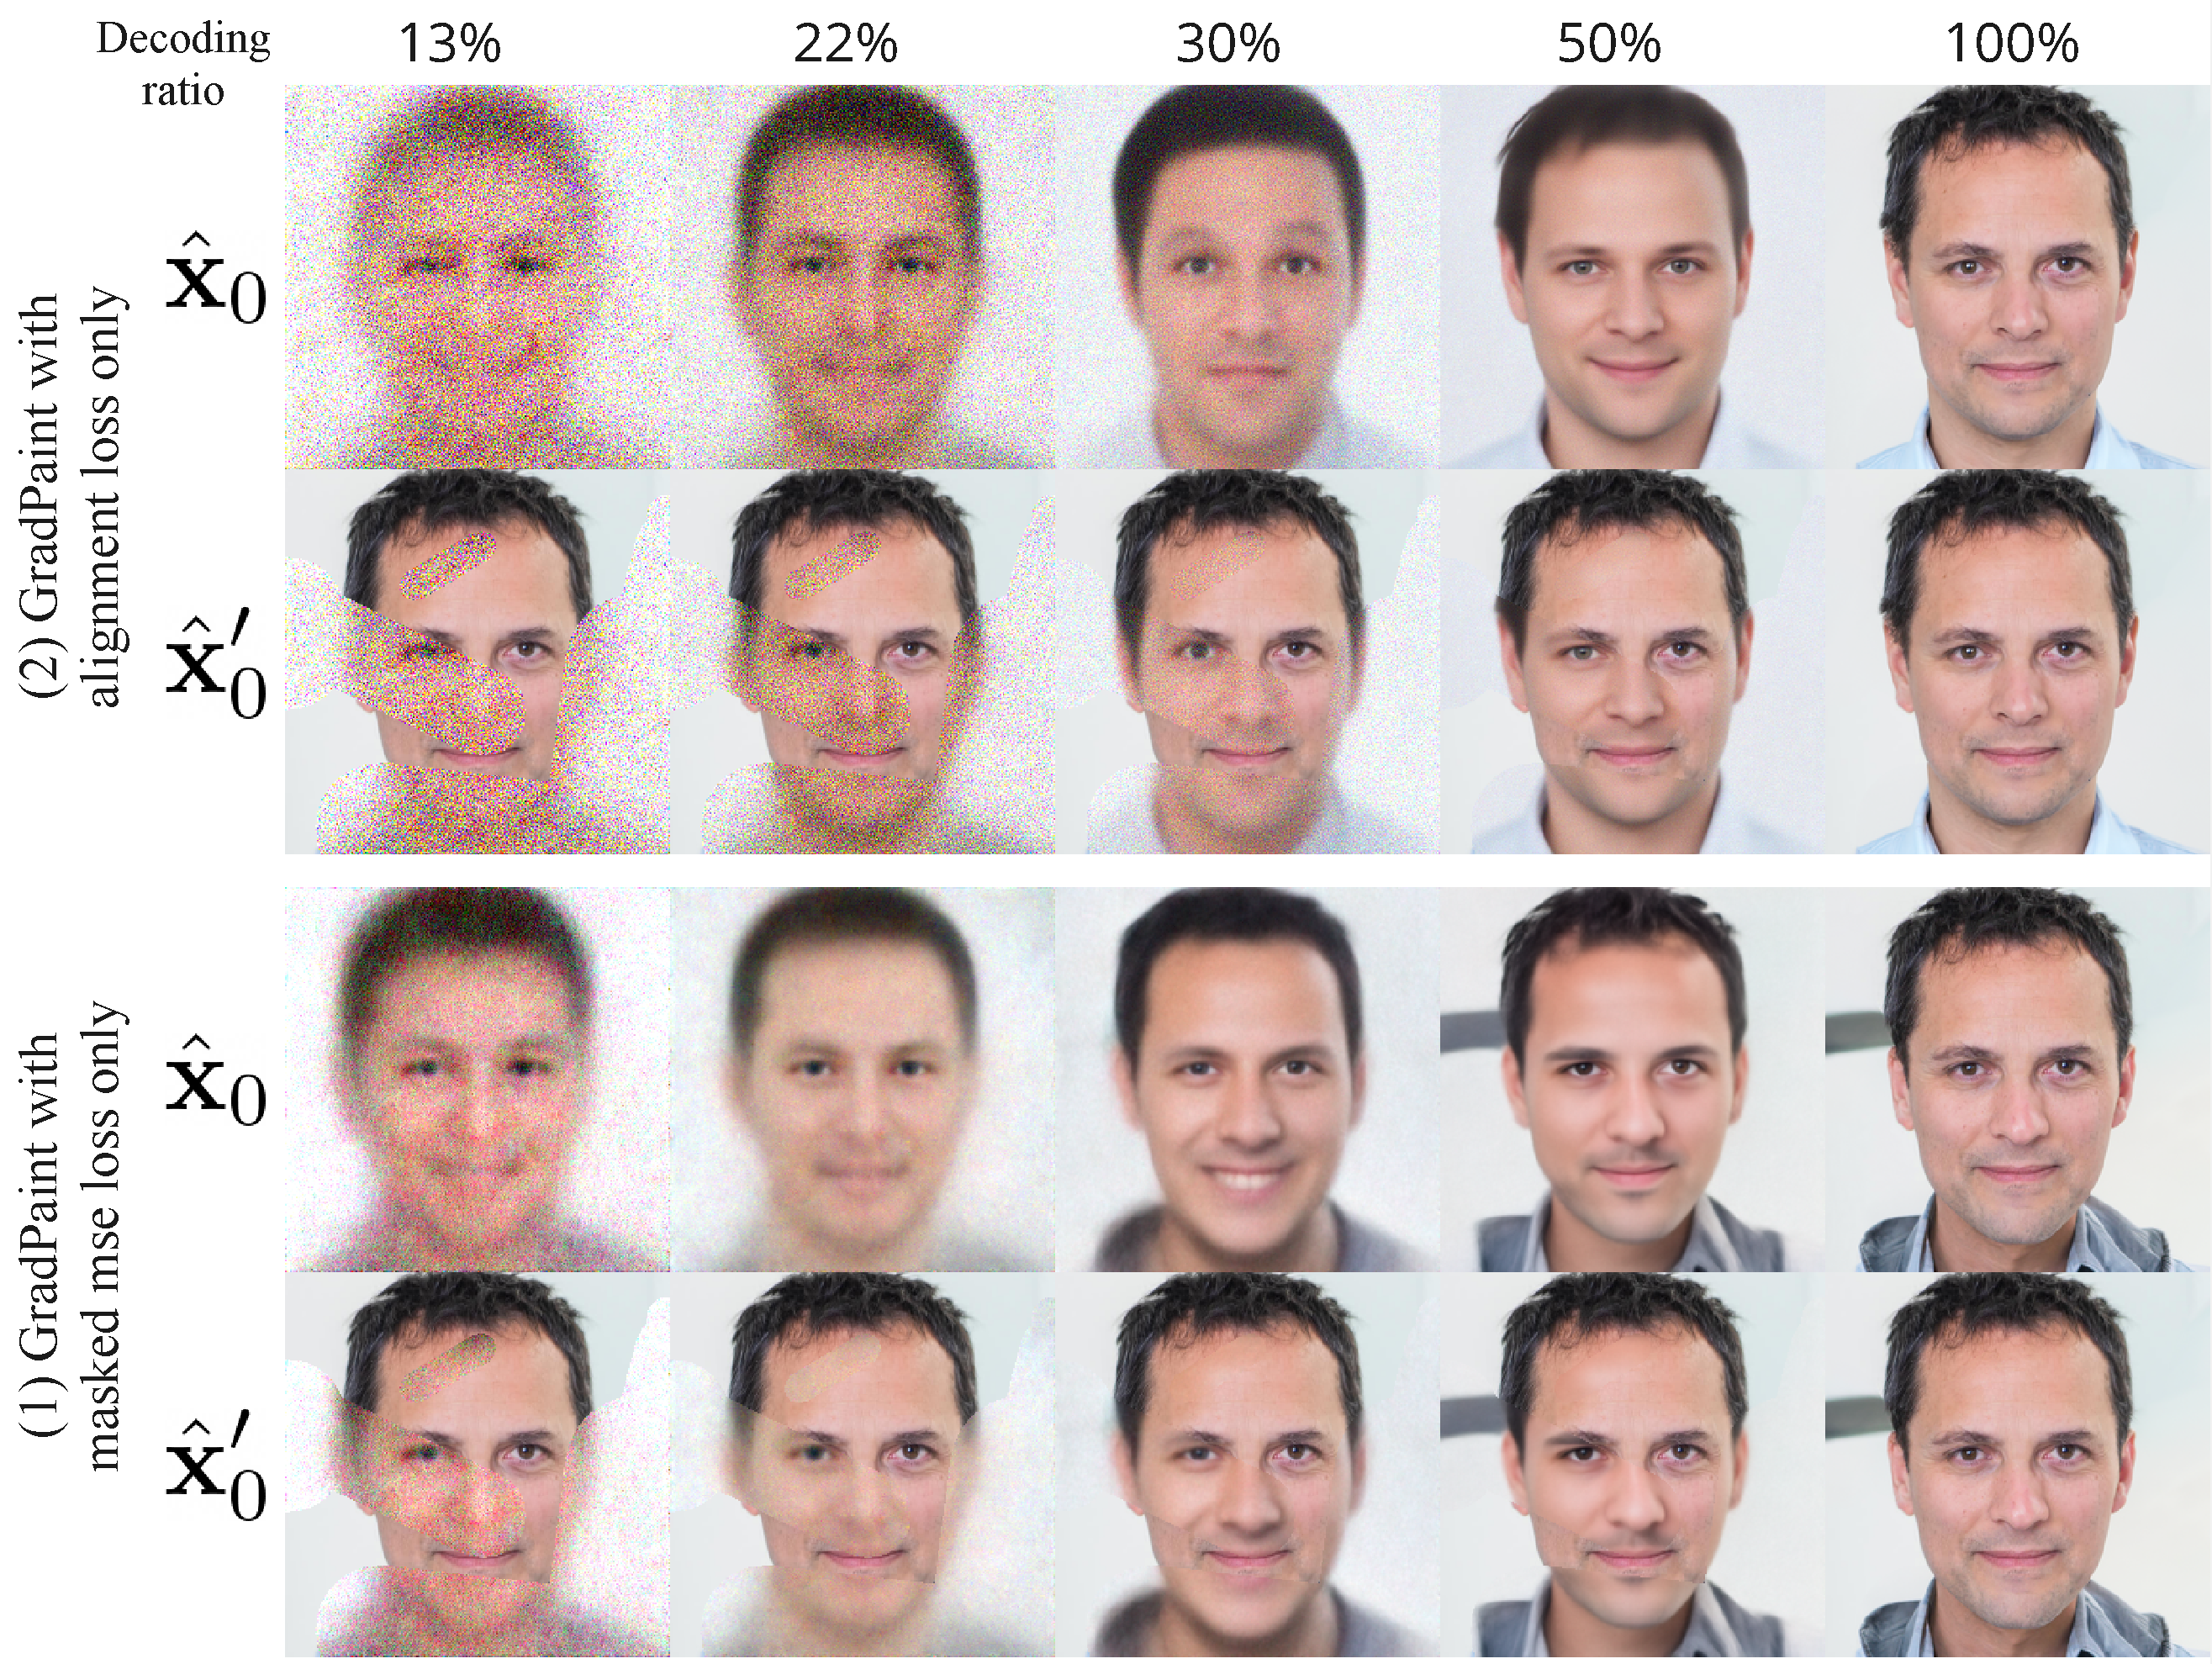
\includegraphics[width=0.8\linewidth]{images/gradpaint/losses1.pdf}
%     \caption{Intermediate DDPM predictions with GradPaint using separate components of our loss. The alignment loss encourages smooth and coherent transitions, as can be seen with the homologous background.}
%     \label{fig:loss_intuition-int}
%   \end{subfigure}
%   \caption{Effect of separate components of our loss on the intermediate predictions of the DDPM model and their corresponding gradients. Noise maps are initialized identically.}
%   \label{fig:loss_intuition}
% \end{figure*}

\begin{figure}[htbp]
  \centering
    \includegraphics[width=\linewidth]{images/gradpaint/losses2.pdf}
    \caption{Gradient magnitude of different components of our losses with regards to $\x_t$. 
    The alignment loss has a concentrated effect at the border and a more global effect
     compared to the masked MSE loss, but dies out more quickly when it concentrates in a few local spots.}
\label{fig:loss_intuition-grad}
\end{figure}

\begin{figure}[htbp]
  \hspace{-1.5cm}
  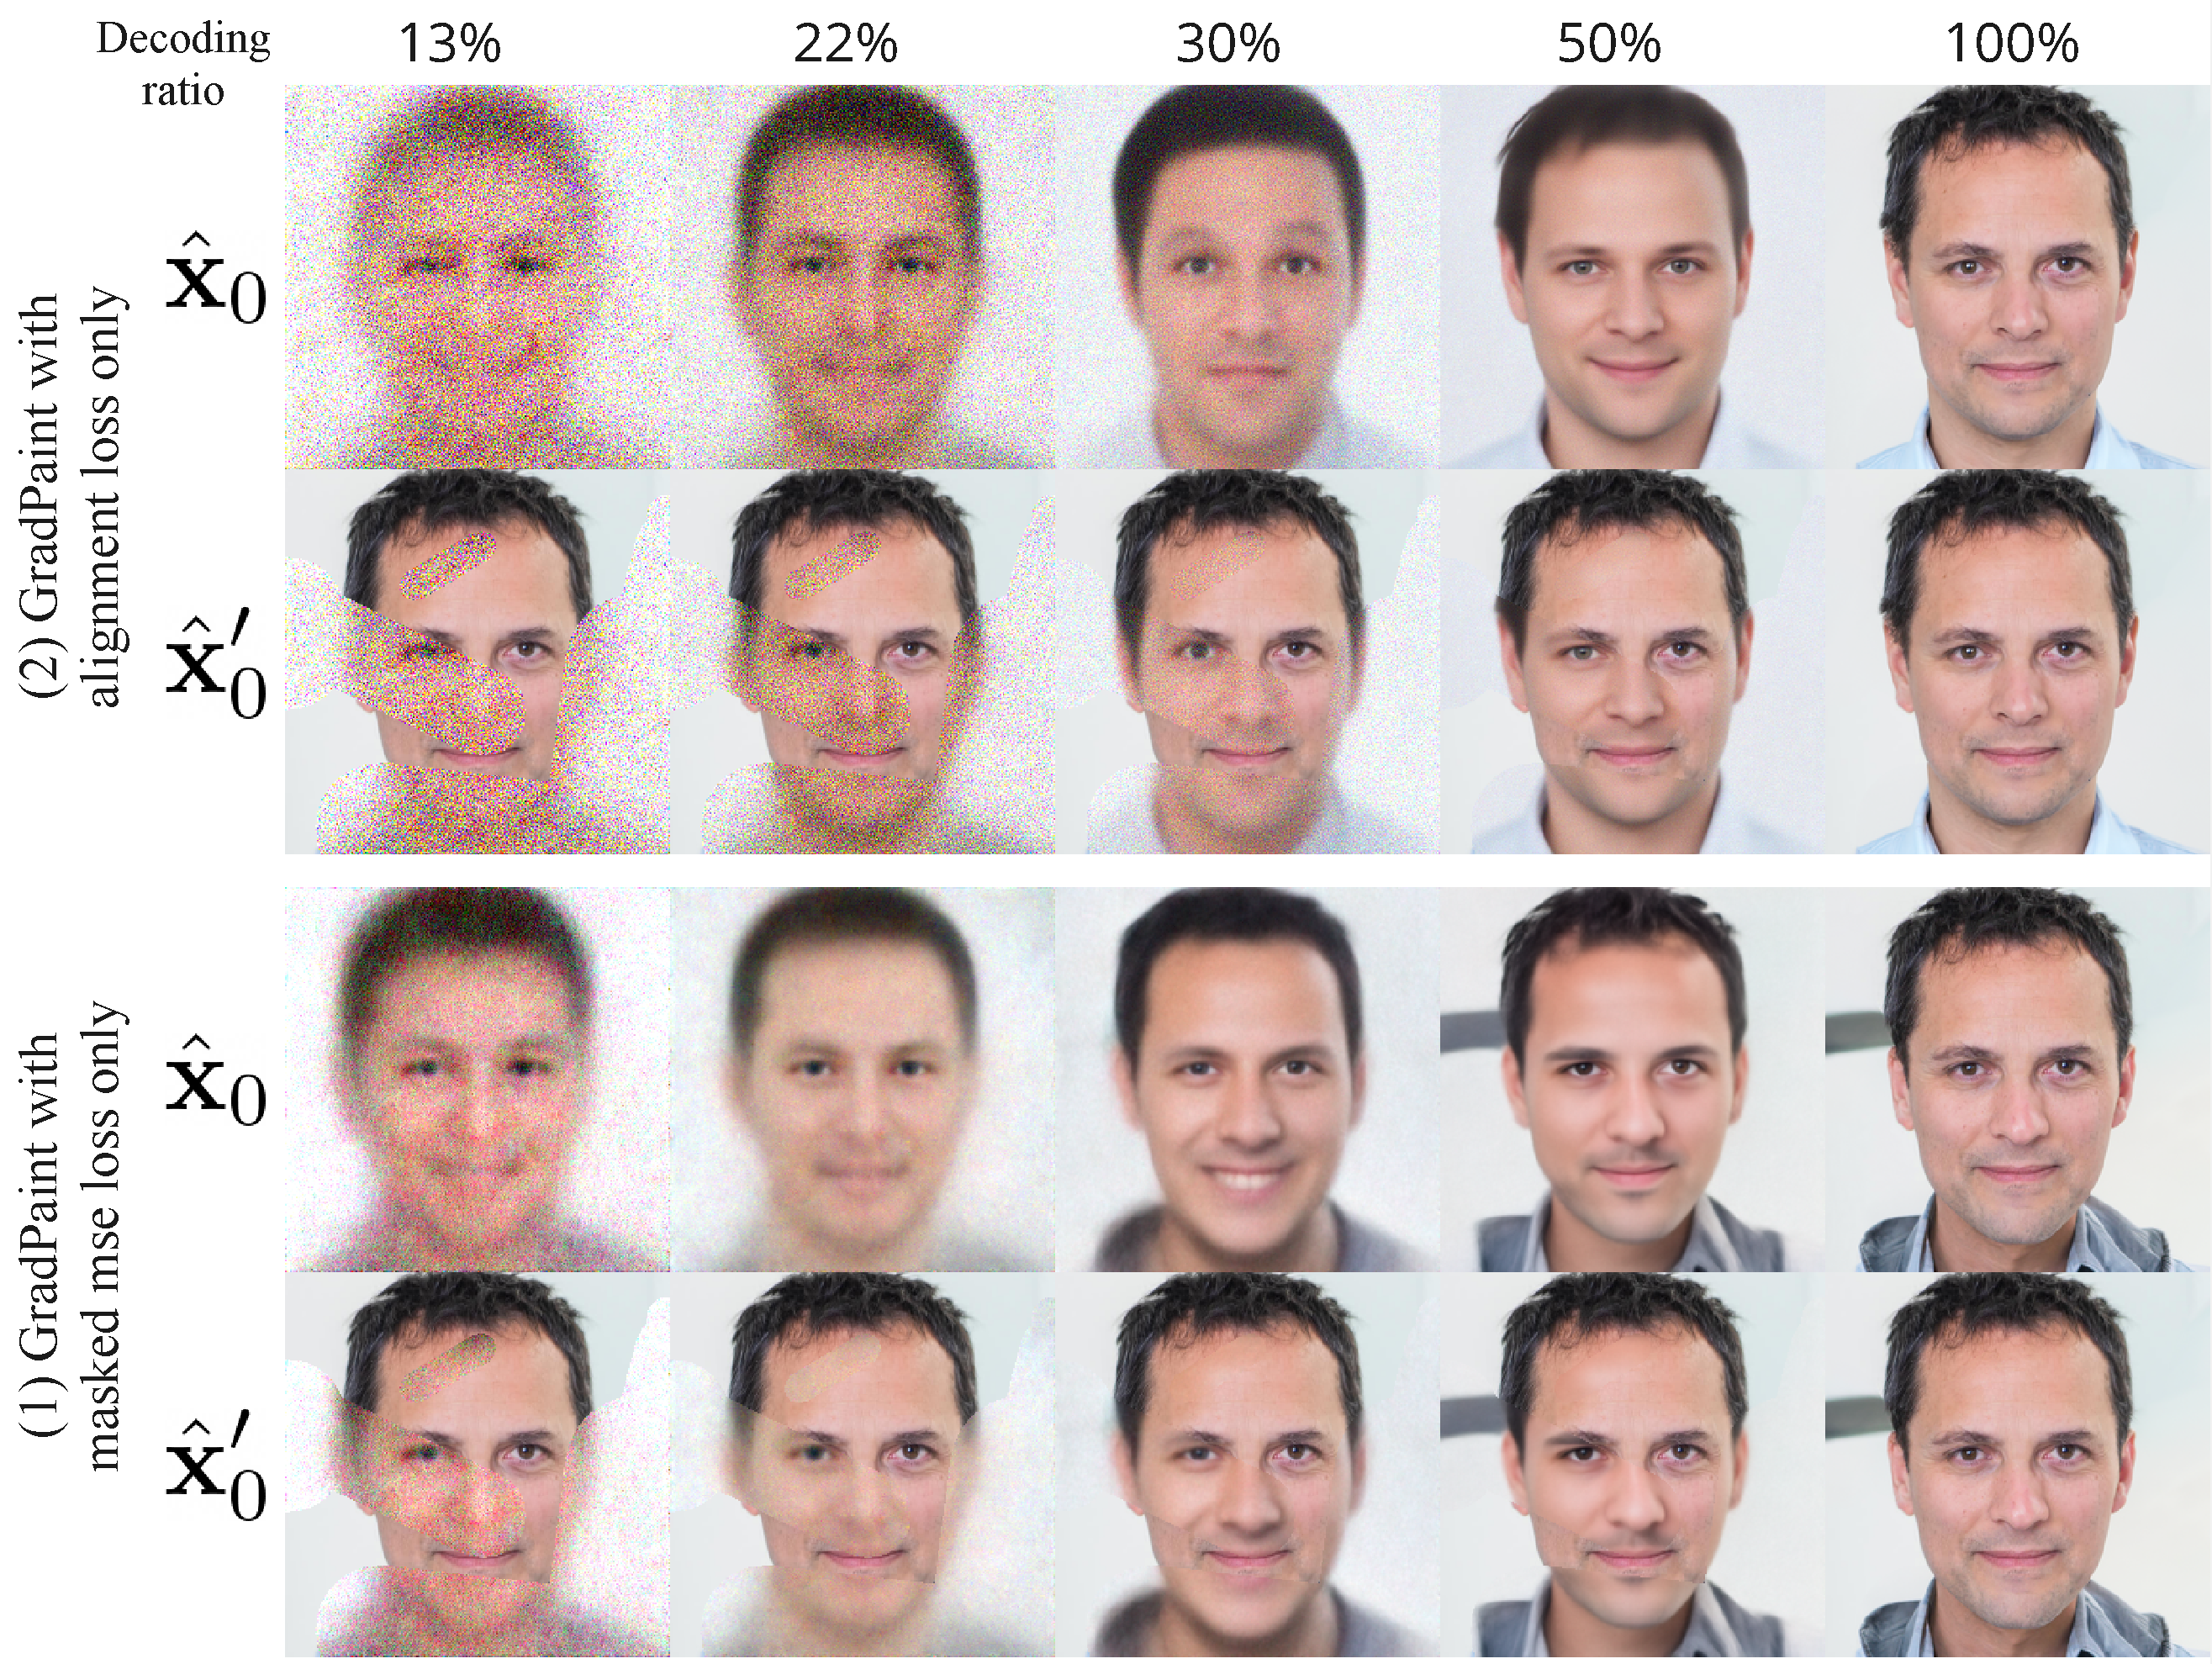
\includegraphics[width=1.2\linewidth]{images/gradpaint/losses1.pdf}
  \caption{Intermediate \ac{DDPM} predictions with GradPaint using separate components of our loss. 
  The alignment loss encourages smooth and coherent transitions, as can be seen with the homologous background.}
\label{fig:loss_intuition-int}
\end{figure}

%   \caption{Effect of separate components of our loss on the intermediate predictions of the DDPM model and their corresponding gradients. Noise maps are initialized identically.}
%   \label{fig:loss_intuition}
% \end{figure*}





% \section{Experimental Results}
%In this section, we describe our experimental setup to compare different algorithms on the inpainting task, and then expose qualitative and quantitative results.
%\subsection{Experiment setup}

\section{Evaluation Protocol}


\subsection{Pre-trained models and implementation details} 
We detail our setup for image-space diffusion models as well as latent-space diffusion models.
We provide a detailed list of the assets 
used in our work (datasets, code, and models) in
the Appendix in~\ref{sec:GradPaint assets}.

\minipar{Experiments on image-space diffusion models}
We primarily use diffusion models from guided diffusion~\citep{dhariwal2021diffusion}, which operates on images of size $256\times256$. 
We use their pre-trained unconditional models (pre-trained on FFHQ, CelebaHQ, and Places2)  as well as their class-conditional model
trained on ImageNet. 

We use a default number of 100 steps for \ac{DDPM} 
sampling; the loss is computed with $\lambda_{al} =400$ during the first 45 steps of decoding (and disabled afterwards following 
our observations shown in~\ref{fig:loss_intuition-grad}). The gradient is updated with a fixed learning rate of $0.005$.


\minipar{Extension to latent diffusion models}

We also experiment with latent diffusion models~\citep{rombach2022high}.  We have observed that the latent spaces that we use have much
 less structure compared to real images, and that our alignment loss, whose role is to enforce smoothness on real images, 
 cannot fulfill this role in latent spaces. Therefore, for all experiments with latent diffusion models, we only experiment with 
 the masked MSE loss, which 
 naturally extends to latent spaces by considering the encoded input image as reference in our MSE loss.

Latent diffusion models also operate on $256\times256$ images, but images are
 edited in a latent space with spatial dimensions of $64\times64$.
 We use pre-trained unconditional latent diffusion models on CelebAHQ and FFHQ. We use the class-conditional 
 latent diffusion model pre-trained on ImageNet. Finally, for text-conditional models, we use Stable Diffusion pre-trained on the 
 public LAION-5B dataset~\citep{schuhmann2022laion}.

 We use a default number of 100 steps for DDPM sampling; the loss is computed with $\lambda_{mse} = 1$.
 The gradient is updated with a fixed learning rate of $0.005$.


\subsection{Datasets}
We evaluate our algorithm on five datasets: FFHQ, CelebaHQ, ImageNet, Places2 and COCO.

Given an image, the aim is to perform inpainting inside a random mask generated with the mask generator from~\cite{lama}. 
We mainly evaluate on the difficult and more realistic \textit{thick} masks, but also provide results for \textit{thin} and 
\textit{medium} masks, like \cite{lama}. We create 5000 masked images for all experiments.

For both image-space and latent diffusion models, we evaluate the FFHQ-pre-trained model on a subset of CelebAHQ masked images. 
Inversely, we evaluate the CelebAHQ pre-trained model on a subset of FFHQ masked images. We evaluate the ImageNet pre-trained 
models on a subset ImageNet validation set and use the class label as conditioning. 

For the image-space diffusion model pre-trained on Places2, we use a subset of the Places2 validation set for evaluation.

Finally, for the Stable Diffusion model pre-trained on LAION-5B, we use a subset of the COCO validation set and use the 
captions as conditioning text information for the diffusion model. 

\subsection{Metrics}

For a set of images inpainted with a given method, we compute two core metrics that encapsulate the challenges
 of inpainting: the LPIPS distance~\citep{zhanglpips2018} between the inpainted image and the (unmasked) input image which measures 
 the extent to which we correctly recover the masked regions, and the FID score~\citep{heusel2017gans} which measures the realism 
 of output images. The primary requirement is that inpainted images should look as natural as possible, hence having the smallest 
 possible FID score. For LPIPS distances, an inpainting result closer to the reference image is generally better, although realistic 
 images further away from the reference image can also be satisfactory, especially for large masks. 


\subsection{Baselines}  We compute the best and worst possible LPIPS and FID scores with two trivial measures: 
the \textit{COPY} oracle measure, which simply copies the (unmasked) input image, gives an LPIPS score of $0$ and a lower bound on 
possible FID scores; and the \textit{GREYFILL} measure, which simply fills the region to be inpainted with uniform grey. 
We also add a \textit{Latent COPY} oracle for latent diffusion models which consists in simply auto-encoding the input image.
Without
 gradient-based optimization, our method is equivalent to the \textit{combine-image} baseline for image inpainting, which we evaluate 
 in our experiments along with its \textit{combine-noisy} variant. Apart from these three closely related methods, we compare against
  the following state-of-the-art inpainting methods:  LaMa~\citep{lama}, a GAN-based method trained for inpainting; 
  Palette~\citep{saharia2022palette}, also trained for inpainting but with diffusion models, RePaint~\citep{lugmayr2022repaint}, another
   training-free inpainting algorithm that is much more computationally expensive, and finally MCG~\citep{mcg}, a parallel line 
   of work to ours which is similarly training-free but with a different optimization scheme. 


\section{Quantitative results}


\begin{table*}[t]
  \hspace{-1cm}
  \scriptsize
  \begin{tabular}{|l|c|c|c|c|c|c|c|c|c|c|c|c|}
  \hline
  \multicolumn{1}{|r|}{Dataset} &
    \multicolumn{6}{c|}{FFHQ} &
    \multicolumn{6}{c|}{CelebaHQ} \\ \hline
  \multicolumn{1}{|r|}{Masks} &
    \multicolumn{2}{c|}{Thin} &
    \multicolumn{2}{c|}{Medium} &
    \multicolumn{2}{c|}{Thick} &
    \multicolumn{2}{c|}{Thin} &
    \multicolumn{2}{c|}{Medium} &
    \multicolumn{2}{c|}{Thick} \\ \hline
  
  \multicolumn{1}{|r|}{Metrics} &
    \multicolumn{1}{c|}{FID$\downarrow$} &
    \multicolumn{1}{c|}{LPIPS$\downarrow$} &
    \multicolumn{1}{c|}{FID$\downarrow$} &
    \multicolumn{1}{c|}{LPIPS$\downarrow$} &
    \multicolumn{1}{c|}{FID$\downarrow$} &
    \multicolumn{1}{c|}{LPIPS$\downarrow$} &
    \multicolumn{1}{c|}{FID$\downarrow$} &
    \multicolumn{1}{c|}{LPIPS$\downarrow$} &
    \multicolumn{1}{c|}{FID$\downarrow$} &
    \multicolumn{1}{c|}{LPIPS$\downarrow$} &
    \multicolumn{1}{c|}{FID$\downarrow$} &
    \multicolumn{1}{c|}{LPIPS$\downarrow$}  \\ \hline
  
    \rowcolor[gray]{0.7}
  COPY (oracle) &
    \multicolumn{1}{c|}{4.29} &
    \multicolumn{1}{c|}{0} &
    \multicolumn{1}{c|}{4.29} &
    \multicolumn{1}{c|}{0} &
    \multicolumn{1}{c|}{4.29} &
    \multicolumn{1}{c|}{0} &
    \multicolumn{1}{c|}{3.01} &
    \multicolumn{1}{c|}{0} &
    \multicolumn{1}{c|}{3.01} &
    \multicolumn{1}{c|}{0} &
    \multicolumn{1}{c|}{3.01} &
    \multicolumn{1}{c|}{0} \\ \hline
  GREYFILL &
    \multicolumn{1}{c|}{154.6} &
    \multicolumn{1}{c|}{0.353} &
    \multicolumn{1}{c|}{98.75} &
    \multicolumn{1}{c|}{0.250} &
    78.08 &
    0.257
    &
    \multicolumn{1}{c|}{173.65} &
    \multicolumn{1}{c|}{0.3770} &
    \multicolumn{1}{c|}{124.32} &
    \multicolumn{1}{c|}{0.2631} &
    96.41 &
    0.264
     \\ \Xhline{4\arrayrulewidth}
  LaMa&
    \multicolumn{1}{c|}{\textbf{6.22}} &
    \multicolumn{1}{c|}{\textbf{0.041}} &
    \multicolumn{1}{c|}{{\underline{5.61}}} &
    \multicolumn{1}{c|}{\textbf{0.052}} &
    6.27 &
    \textbf{0.076}
     &
    \multicolumn{1}{c|}{n/a} &
    \multicolumn{1}{c|}{n/a} &
    \multicolumn{1}{c|}{n/a} &
    \multicolumn{1}{c|}{n/a} &
    \multicolumn{1}{c|}{n/a} &
    \multicolumn{1}{c|}{n/a} \\ \hline
  Palette &
    \multicolumn{1}{c|}{6.78} &
    \multicolumn{1}{c|}{{\underline{0.049}}} &
    \multicolumn{1}{c|}{6.78} &
    \multicolumn{1}{c|}{{\underline{0.068}}} &
    \multicolumn{1}{c|}{7.28} &
    \multicolumn{1}{c|}{0.096}
    &
    \multicolumn{1}{c|}{n/a} &
    \multicolumn{1}{c|}{n/a} &
    \multicolumn{1}{c|}{n/a} &
    \multicolumn{1}{c|}{n/a} &
    \multicolumn{1}{c|}{n/a} &
    \multicolumn{1}{c|}{n/a} \\ \Xhline{4\arrayrulewidth}
  Repaint &
    \multicolumn{1}{c|}{13.25} &
    \multicolumn{1}{c|}{0.060} &
    \multicolumn{1}{c|}{12.21} &
    \multicolumn{1}{c|}{0.080} &
    \multicolumn{1}{c|}{9.09} &
    \multicolumn{1}{c|}{0.090} &
    \multicolumn{1}{c|}{8.23} &
    \multicolumn{1}{c|}{\textbf{0.047}} &
    \multicolumn{1}{c|}{8.14} &
    \multicolumn{1}{c|}{\underline{0.062}} &
    \multicolumn{1}{c|}{8.44} &
    \multicolumn{1}{c|}{\textbf{0.078}}  \\ \hline
  MCG &
    \multicolumn{1}{c|}{7.71} &
    \multicolumn{1}{c|}{0.062} &
    \multicolumn{1}{c|}{5.97} &
    \multicolumn{1}{c|}{0.073} &
    \multicolumn{1}{c|}{\underline{6.17}} &
    \multicolumn{1}{c|}{0.097}
    &
    \multicolumn{1}{c|}{8.43} &
    \multicolumn{1}{c|}{0.059} &
    \multicolumn{1}{c|}{6.52} &
    \multicolumn{1}{c|}{0.065} &
    \multicolumn{1}{c|}{6.67} &
    \multicolumn{1}{c|}{0.084} \\ \hline
  \begin{tabular}[c]{@{}l@{}}\textit{combine-noisy}\end{tabular} &
    \multicolumn{1}{c|}{13.48} &
    \multicolumn{1}{c|}{0.090} &
    \multicolumn{1}{c|}{9.35} &
    \multicolumn{1}{c|}{0.099} &
    \multicolumn{1}{c|}{9.04} & 
    \multicolumn{1}{c|}{0.119}
     &
    \multicolumn{1}{c|}{ 11.1} &
    \multicolumn{1}{c|}{0.070} &
    \multicolumn{1}{c|}{9.78} &
    \multicolumn{1}{c|}{0.081} &
    \multicolumn{1}{c|}{9.89} & 
    \multicolumn{1}{c|}{0.103}
     \\ \hline
  \begin{tabular}[c]{@{}l@{}}\textit{combine-image}\end{tabular} &
    \multicolumn{1}{c|}{11.19} &
    \multicolumn{1}{c|}{0.096} &
    \multicolumn{1}{c|}{7.49} &
    \multicolumn{1}{c|}{0.102} &
    \multicolumn{1}{c|}{7.30} &
    \multicolumn{1}{c|}{0.123}
     &
    \multicolumn{1}{c|}{\underline{7.89}} &
    \multicolumn{1}{c|}{0.080} &
    \multicolumn{1}{c|}{\underline{5.96}} &
    \multicolumn{1}{c|}{0.089} &
    \multicolumn{1}{c|}{\underline{5.83}} &
    \multicolumn{1}{c|}{0.110}\\ \hline
  GradPaint (ours) &
    \multicolumn{1}{c|}{{\underline{6.613}}} &
    \multicolumn{1}{c|}{0.060} &
    \multicolumn{1}{c|}{\textbf{5.39}} &
    \multicolumn{1}{c|}{{\underline{0.069}}} &
    \multicolumn{1}{c|}{\textbf{5.65}} &
    \multicolumn{1}{c|}{{\underline{0.084}}}
     &
    \multicolumn{1}{c|}{\textbf{5.13}} &
    \multicolumn{1}{c|}{{\underline{0.051}}} &
    \multicolumn{1}{c|}{\textbf{4.29}} &
    \multicolumn{1}{c|}{\textbf{0.059}} &
    \multicolumn{1}{c|}{\textbf{4.41}} &
    \multicolumn{1}{c|}{\textbf{0.077}} \\ \hline
  \end{tabular}
   
  \caption{Evaluation of various methods on FFHQ and CelebaHQ datasets. 
  The COPY oracle and the GREYFILL measure are respectfully the lower and 
  upper bounds for LPIPS and FID. LaMa and Palette are both training-based methods. 
  RePaint, \emph{combine-noisy}, \emph{combine-image}, MCG and GradPaint are all 
  training-free methods which all use the same model based on guided diffusion~\citep{dhariwal2021diffusion}. 
  Best score is shown \textbf{in bold} and second best \underline{underlined}.}
  \label{main_results}
  \end{table*}

  \begin{table}
    \centering
    \begin{tabular}{|c|l|l|}
    \hline
    Method                                                                  & FID $\downarrow$           & LPIPS $\downarrow$           \\ \hline
    \textit{combine-noisy}                                                  & 10.33         & 0.1907          \\ \hline
    \textit{combine-image}                                                  & 9.61          & 0.1797          \\ \hline
    \begin{tabular}[c]{@{}c@{}}GradPaint \\ w/o alignment loss\end{tabular} & 8.12          & 0.1551          \\ \hline
    GradPaint                                                               & \textbf{7.86} & \textbf{0.1486} \\ \hline
    \end{tabular}
    \caption{Detailed comparison on ImageNet pre-trained guided diffusion model with \emph{thick} masks.}%
    \label{tab:quantitative_ablation}
  \end{table}

  \vspace{1cm}

    

% \begin{table}
% \begin{minipage}[t]{.60\linewidth}\vspace*{0pt}%
%     \footnotesize
%     \begin{tabular}{|c|l|l|}
% \hline
% Method                                                                  & FID $\downarrow$           & LPIPS $\downarrow$           \\ \hline
% \textit{combine-noisy}                                                  & 10.33         & 0.1907          \\ \hline
% \textit{combine-image}                                                  & 9.61          & 0.1797          \\ \hline
% \begin{tabular}[c]{@{}c@{}}GradPaint \\ w/o alignment loss\end{tabular} & 8.12          & 0.1551          \\ \hline
% GradPaint                                                               & \textbf{7.86} & \textbf{0.1486} \\ \hline
% \end{tabular}
% \end{minipage}
% \hfill
% \begin{minipage}[t]{.35\linewidth}
%     \setlength{\abovecaptionskip}{0pt}%
%     \caption{Detailed comparison on ImageNet pre-trained guided diffusion model with \emph{thick} masks.}%
%     \label{tab:quantitative_ablation}
% \end{minipage}
% \end{table}


\subsection{Image-space Diffusion Models}

Quantitative results on the FFHQ and CelebA datasets for image-space diffusion models are shown in Tab.~\ref{main_results}, 
where GradPaint is compared against 
available competing methods (FFHQ-pretrained checkpoints are not available for Palette and LAMA) as well as the \textit{combine} 
baselines. We present all mask types, although we argue that the setting with \emph{thick} masks is the most interesting 
setting for practical applications. For \emph{thick masks},
the benefit of our gradient update is visible when comparing to \textit{combine-image}
(same as ours without gradient updates): On FFHQ, the FID score is reduced from 7.30 to 5.65, a significant improvement given that 
the minimum obtainable FID score is 4.29 on 5000 images (\textit{COPY} oracle measure). Results on both datasets show similar gains. 
When comparing with competing methods on FFHQ, GradPaint obtains the state-of-the art FID score, outperforming methods specialized in 
inpainting (Palette, LAMA) as well as the training-free algorithms Repaint and MCG based on the same diffusion model as ours. LaMa 
obtains slightly better LPIPS scores but requires an inpainting-specific training (compared to simply using a pre-trained generative 
model). For \emph{thin} and \emph{medium} masks, our method also  generally achieves the best FID score 
and a comparable LPIPS score even with LaMa's fully supervised method. Moreover, LaMa, unlike all other methods, 
has access at train time to the mask distribution that we use for testing.  



We validate different components of our method with the ImageNet~\citep{deng2009imagenet} dataset and  guided diffusion model, summarized in 
Tab.~\ref{tab:quantitative_ablation}. This more difficult dataset was chosen to better analyze our different components as well as 
validate our method on class-conditioned diffusion models, where generation could be biased by the class. Our full method, and the 
alignment loss in particular, improves reconstruction and realism of generated images.


% Finally, Tab.~\ref{inference_time} summarizes main results on FFHQ, algorithm type (training-based or training-free) and inference time for different methods. We see that the gradient-based update incurs an additional cost for inpainting images: GradPaint is roughly 3x slower than the \textit{combine-image} reference method. However, when we adapt GradPaint to work in latent image spaces and use a latent diffusion model, the inference time is reduced to just 7.2s per image, while still maintaining better FID score (5.97) than competing methods. Details on adapting GradPaint to latent diffusion models are presented in the next section.


% Please add the following required packages to your document preamble:
% \usepackage{multirow}
\begin{table}[h]
\centering
\begin{tabular}{|r|cc|cc|cc|cc|cc|}
\hline
Dataset &
  \multicolumn{2}{c|}{ImageNet} &
  \multicolumn{2}{c|}{COCO} &
  \multicolumn{2}{c|}{FFHQ}  \\ \hline
  
\multicolumn{1}{|c|}{} &
  \multicolumn{1}{c|}{FID $\downarrow$} &
  LPIPS $\downarrow$ &
  \multicolumn{1}{c|}{FID $\downarrow$} &
  LPIPS $\downarrow$ &
  \multicolumn{1}{c|}{FID $\downarrow$} &
  LPIPS $\downarrow$ \\ \hline
  \rowcolor[gray]{0.7}
COPY (o.) &
  \multicolumn{1}{c|}{12.27} &
  0.0 &
  \multicolumn{1}{c|}{7.29} &
  0.0 &
  \multicolumn{1}{c|}{4.29} &
  0.0
  \\ \hline
  \rowcolor[gray]{0.7}
Lat. COPY (o.) &
  \multicolumn{1}{c|}{12.00} &
  0.034 &
  \multicolumn{1}{c|}{7.71} &
  0.041 &
  \multicolumn{1}{c|}{4.98} &
  0.018
  \\ \hline
GREYFILL &
  \multicolumn{1}{c|}{34.51} &
  0.269 &
  \multicolumn{1}{c|}{29.97} &
  0.264 &
  \multicolumn{1}{c|}{77.43} &
  0.257 \\ \Xhline{4\arrayrulewidth}
\begin{tabular}[c]{@{}r@{}}\textit{combine-noisy}\end{tabular} &
  \multicolumn{1}{c|}{17.17} &
  0.195 &
  \multicolumn{1}{c|}{11.12} &
  0.241  &
  \multicolumn{1}{c|}{8.73} &
  0.132 
  \\ \hline
\begin{tabular}[c]{@{}r@{}}\textit{combine-image}\end{tabular} &
  \multicolumn{1}{c|}{17.37} &
  0.207 &
  \multicolumn{1}{c|}{12.68} &
  0.257 &
  \multicolumn{1}{c|}{6.832} &
  0.127
  \\ \hline
\begin{tabular}[c]{@{}r@{}}GradPaint\\ (ours)\end{tabular} &
  \multicolumn{1}{c|}{\textbf{14.62}} &
  \textbf{0.163} &
  \multicolumn{1}{c|}{\textbf{9.43}} &
  \textbf{0.216} &
  \multicolumn{1}{c|}{\textbf{5.97}} &
  \textbf{0.111}\\ \hline
\end{tabular}
\caption{Evaluation of pre-trained latent diffusion models with \emph{thick} masks. The COPY oracle measures the metrics on the ground-truth images, and the Latent COPY oracle does the same for autoencoded ground-truth images. As we can see, our modification for latent diffusion models yields significant improvements on all datasets.}
\label{latent_table} 
\end{table}





%\newpage
\subsection{Latent Diffusion Models}

 Results on Latent Diffusion Models are presented in Tab.~\ref{latent_table}. As we can see, the latent space allows for very good image 
 reconstruction (small LPIPS scores), so it is not a real limitation and GradPaint (latent) is still able to outperform competing 
 methods (FID 5.97 on FFHQ \emph{thick} masks). Overall, we observe large and consistent gains on all three datasets ImageNet, 
 COCO and FFHQ datasets over the reference inpainting methods, for both FID and LPIPS.





\section{Qualitative results}

\subsection{Image-space Diffusion Models}

Figs.~\ref{fig:places} and~\ref{fig:res2} and  show qualitative results using our method for Places2 and ImageNet pre-trained models, 
respectfully. Note that without the gradient-guidance of GradPaint, generations are unable to harmonize well.
Images produced by RePaint~\citep{lugmayr2022repaint} often lack global coherence, like the missing spider web in Fig.~\ref{fig:res2}. 
Our method produces globally and locally harmonized images, without the heavy computation cost of~\cite{lugmayr2022repaint} nor the 
specific supervised training of \cite{lama}. Note that we selected images where the \textit{thick} masks masked out key parts 
of the input image to better appreciate the different results.

Fig.~\ref{fig:vis_ablation} shows qualitative results on ImageNet-trained 
 guided diffusion model for different components of our method. We note that the baseline \emph{combine-image} is
  biased by the class-conditioning of the model without taking into account the context, like for the ``red wolf" class. 
  Adding gradient update as well as the alignment loss produces generations harmonized with the surrounding context. 








    \begin{figure}[H]
      \hspace{-2cm} 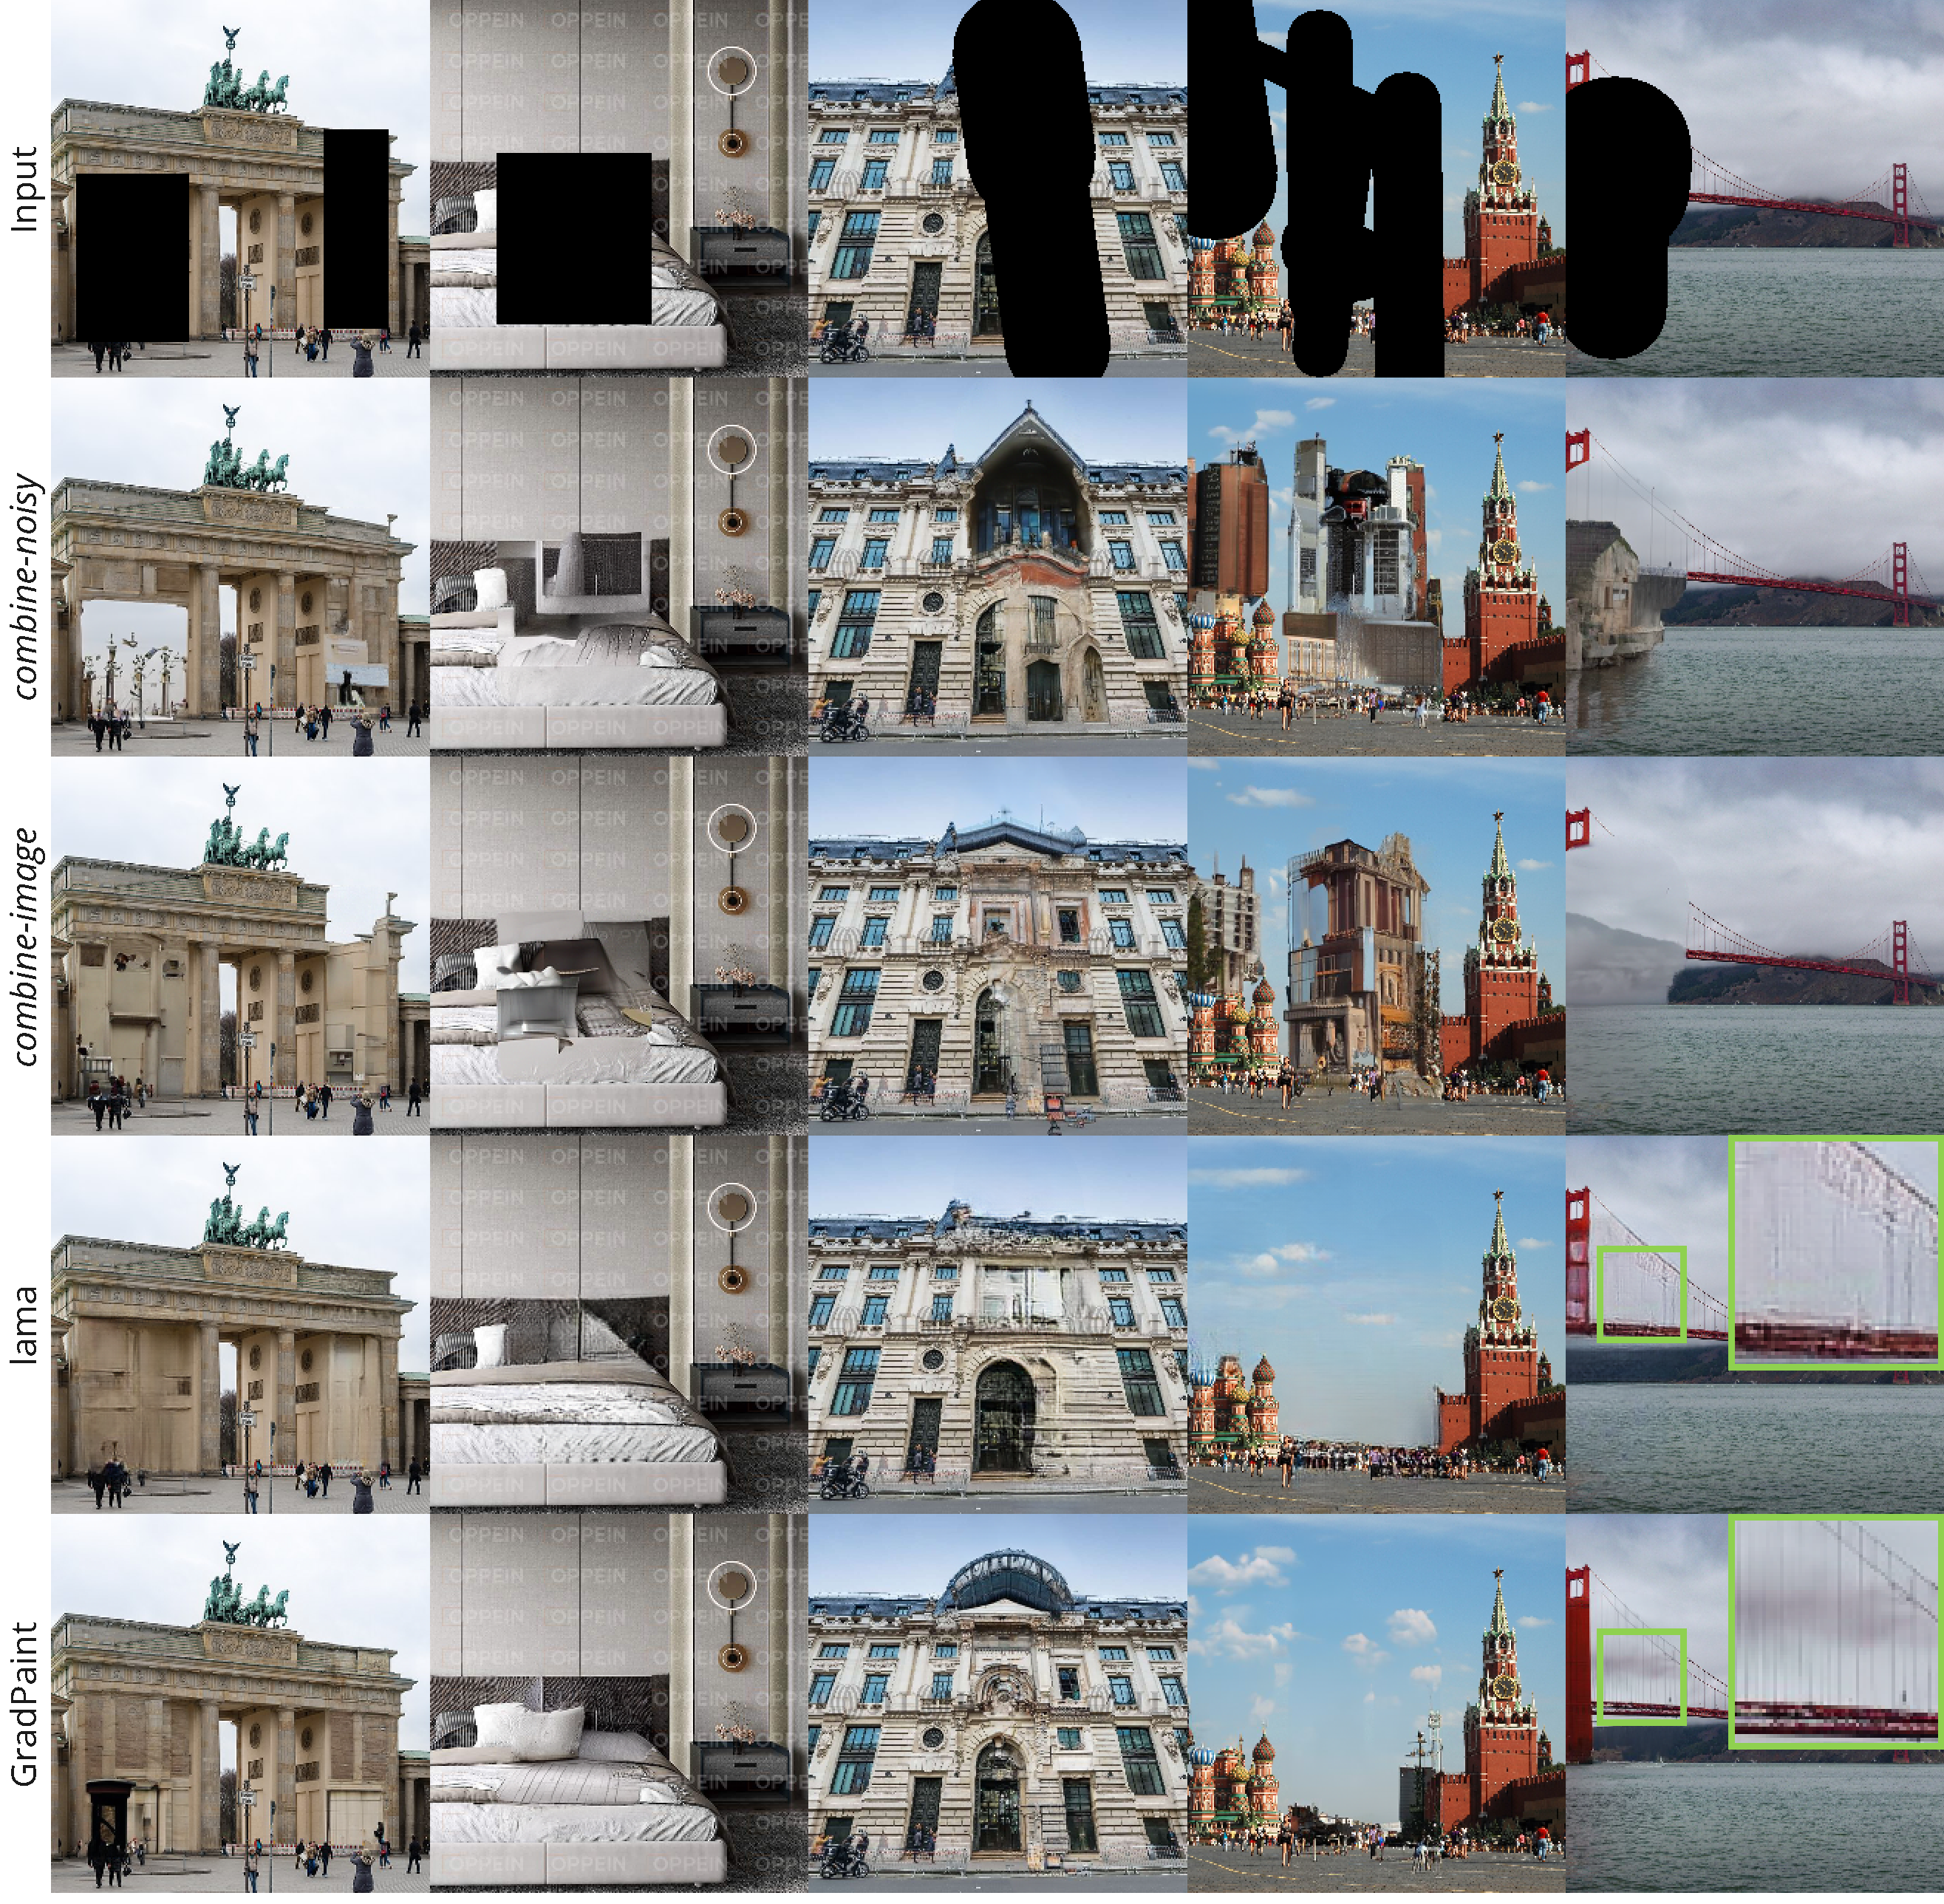
\includegraphics[width=1.2\linewidth]{images/gradpaint/places2.pdf} % tried 1.4
      \caption{In-the-wild images for models trained on Places2. Note that \emph{combine-image}, \emph{combine-noisy} and GradPaint all use the same noise map for initialization. Note that LaMa was specifically trained using similar masks, contrary to our method.}
      \label{fig:places}
    \end{figure}
  
  \begin{figure}[H]
    \centering
      \includegraphics[width=0.8\linewidth]{images/gradpaint/imagenet_results.pdf} %tried 1, too big
      \caption{Inpainting results on select images from ImageNet. The \emph{combine-image} baseline produces unharmonized results and struggles to take the context into account. Our method produces high-quality results at a fraction of the time of RePaint~\citep{lugmayr2022repaint}. }
      \label{fig:res2}
  \end{figure}
  
  
  \begin{figure}[H]
    \centering
    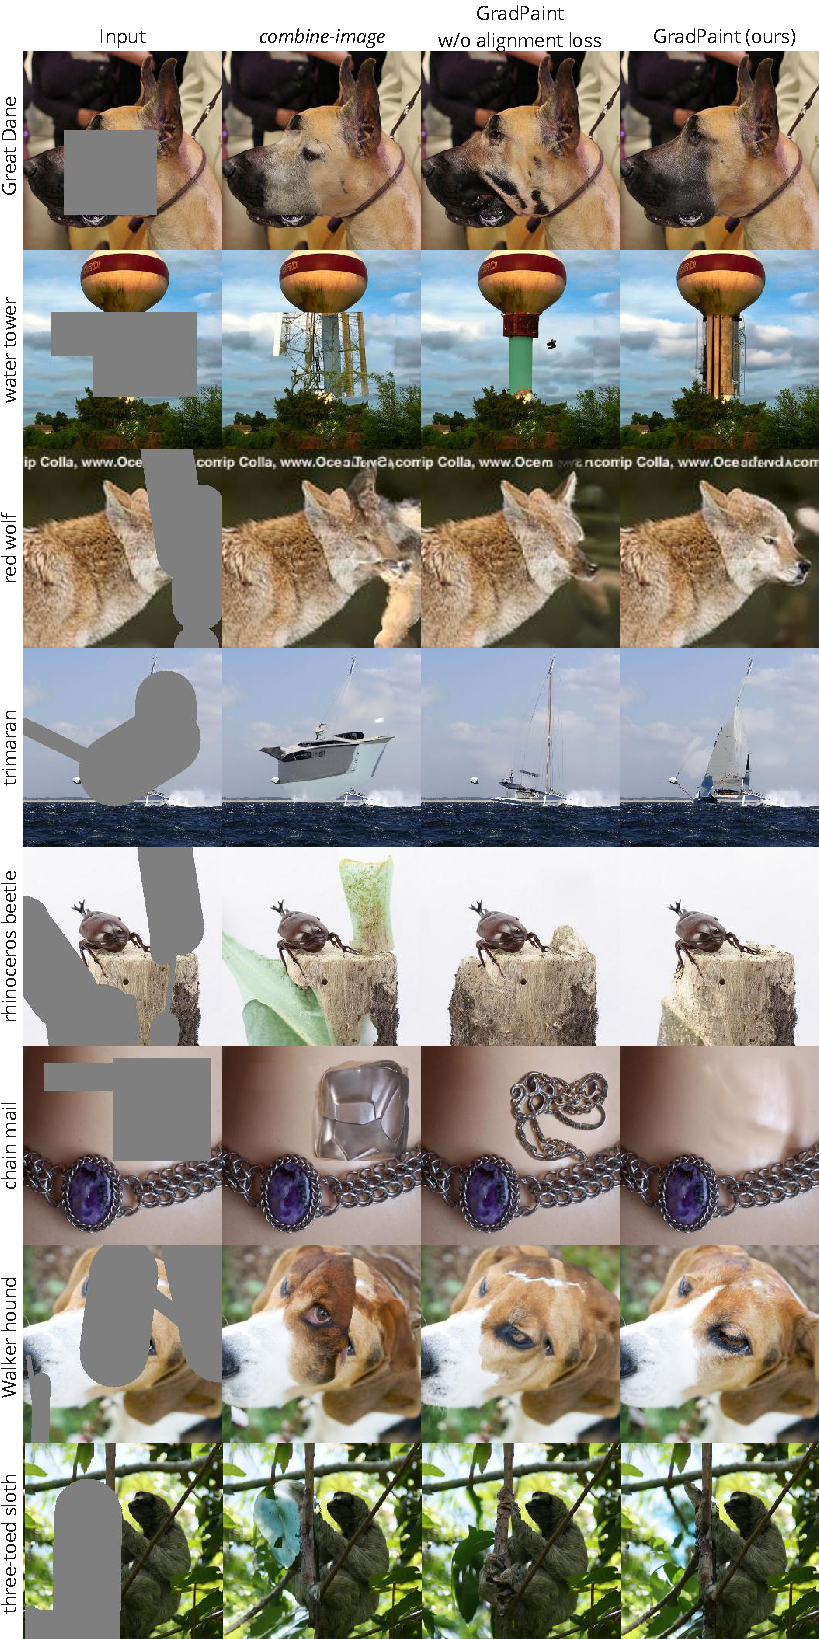
\includegraphics[width=0.75\linewidth]{images/gradpaint/vis_ablation.pdf}
    \caption{Qualitative results for select images of ImageNet dataset. Baseline \emph{combine-image} produces  images with visible artifacts. Our gradient update using only the masked MSE loss improves the ``copy-paste" effect, while the alignment loss produces better aligned transitions.}
    \label{fig:vis_ablation}
  \end{figure}



Figs.~\ref{fig:qualitative_thin} and ~\ref{fig:qualitative_thick} show additional qualitative examples using
\emph{thin} and \emph{medium} masks. With these smaller masks, the visual differences are sometimes harder to 
appreciate, and we recommend zooming when viewing results. We compare our method to the baselines 
\emph{combine-image}, \emph{combine-noisy}, LaMa, and RePaint. Baselines \emph{combine-noisy} and
 \emph{combine-image} clearly have harmonization issues. LaMa tends to have blurry artifacts typical of
  GANs in the generated areas. RePaint generally produces realistic generations, but which aren't always
   coherent with other elements of the image. Our method produces high-quality results at a much smaller
    computational cost than RePaint.


       

    \begin{figure}[H]
      \centering
      \includegraphics[width=\linewidth]{images/gradpaint/ThinMasks.pdf} %tried with 1
        \caption{Qualitative results with thin masks. Best viewed zoomed and in color. 
        In \emph{(a)}, notice the quality of the text of the hat and the background face on the right in \emph{(b)}. 
        Finally, in \emph{(c)}, \emph{(d)}, and \emph{(e)}, methods \emph{combine-noisy} and \emph{combine-image} 
        have harmonization issues (see eyes, cheek/eyebrow, and lips respectively), while our method is on par with the costly RePaint.}
    \label{fig:qualitative_thin}
    \end{figure}
    
    \begin{figure}[H]
      \centering
      \includegraphics[width=\linewidth]{images/gradpaint/MediumMasks.pdf}
        \caption{Qualitative results with medium masks. Best viewed zoomed and in color. Methods \emph{combine-noisy} and \emph{combine-image} have harmonization issues, particularly in \emph{(a)} and \emph{(b)}. Notice the badge on the hat in \emph{(c)} where most methods fail to realistically integrate it with the hat. In \emph{(d)}, our method most successfully generates an eye which matches with the input eye. Finally, all methods struggle with the difficult example \emph{(e)}, as it is poorly represented in the training distriubtion.  Nevertheless, our method is the sole one which attempts to reconstruct the hand as a separate entity from the face.}
    \label{fig:qualitative_thick}
    \end{figure}



    Fig.~\ref{fig:res_ffhq} shows additional select examples on FFHQ dataset. Notice that LaMa produces results
    close to the reference image, but generally containing blurry artifacts, explaining the generally higher
     LPIPS scores but lower FID scores than our method. RePaint's method, despite requiring over 5 minutes of 
     compute time for a generation, produces smooth local changes but often fails to harmonize with the global
      structure of the image (rows 1, 2, 4, 5). Our method produces high-quality and harmonized results, especially
       visible when the generation requires surrounding context, such as rows 1 and 5 which necessitate generating glasses.
 

    %will be displayed next page
\begin{figure}[H]
  \centering
  \includegraphics[width=0.7\linewidth]{images/gradpaint/CVPR_ffhq.jpeg}
  \caption{Results on select images from FFHQ. All models were trained on CelebAHQ dataset.
  While the overall reconstruction of LaMa is decent, zooming on the image unveils 
  visible artifacts typical of \ac{GAN}s. The \emph{combine-image}
   baseline produces images with obvious ``copy/paste" effects. Even 
   with the 4500 forward passes necessary for RePaint, global image coherence often fails.  
   Our method produces a high-quality and harmonized generation.}
\label{fig:res_ffhq}
\end{figure}




 
     Finally, we add an abundant amount of uncurated results to better appreciate our method.
     Figs.~\ref{fig:uncur1}, ~\ref{fig:uncur2}, ~\ref{fig:uncur3}, and ~\ref{fig:uncur4} show uncurated 
     examples from on ImageNet comparing \emph{combine-image}, RePaint, and GradPaint. GradPaint works particularly well when the 
     task requires fine-grained texture alignment (see rows 1, 5, 12, 31)  and tends to work significantly better for global image 
     coherence compared to other methods (see rows 2, 4, 6, 29, 36, 37). However, GradPaint sometimes fails with difficult tasks with 
     unstandard context (see rows 14, 36). From time to time, we see that GradPaint may slightly add unneeded bias to the inpainting 
     task from the background, e.g. row 41 produced a dog with a pink nose, influenced by the pink background. 
  










\begin{figure}[H]
  \centering
    \includegraphics[width=0.75\linewidth]{images/gradpaint/uncur1.jpeg} % tried 0.7
    \caption{Uncurated results on ImageNet (1). Rows 1, 2, 4, 5, 6 display the superior ability of GradPaint to align fine details and global coherence.}
    \label{fig:uncur1}
\end{figure}

\begin{figure}[H]
  \centering
    \includegraphics[width=0.75\linewidth]{images/gradpaint/uncur2.pdf}
    \caption{Uncurated results on ImageNet (2). GradPaint works well on alignement tasks (row 12), but sometimes struggles with non-standard input (row 14). }
    \label{fig:uncur2}
\end{figure}

\begin{figure}[H]
  \centering
    \includegraphics[width=0.75\linewidth]{images/gradpaint/uncur3.jpeg}
    \caption{Uncurated results on ImageNet (3). Our method works well on global coherence (row 29) and generating fine textures requiring alignment (row 31).}
    \label{fig:uncur3}
\end{figure}

\begin{figure}[H]
  \centering
    \includegraphics[width=0.73\linewidth]{images/gradpaint/uncur4.pdf}
    \caption{Uncurated results on ImageNet (4). Our method works well on global coherence (rows 36, 37) but sometimes fails on challenging tasks (row 35). From time to time, the background of the image may poorly influence the content to be generated (row 41).}
    \label{fig:uncur4}
\end{figure}


\subsection{Latent Diffusion Models}

Fig.~\ref{fig:stable_diffusion_qual} shows visual examples of our method using Stable Diffusion on COCO. 
Our method produces realistic and harmonized results compared to the baseline method. 

Finally, Fig.~\ref{fig:qualitative_latent_imagenet} shows visual examples of our inpainting method using 
latent diffusion models on ImageNet. While the baseline method produces low-quality results, our method produces 
realistic and harmonized results.  





\def\myim#1{\includegraphics[width=0.9\textwidth]{images/gradpaint/rebuttal_images/#1}}
\begin{figure}[H]
    \centering
    \renewcommand{\arraystretch}{1} 
    \setlength{\tabcolsep}{27pt} % tried 38; tried 30 ; tried 25
  \begin{tabular}{ccccc}
  
  \hspace{-1cm}Prompt  &  \hspace{-1cm} Original Image & Mask & Baseline & GradPaint \\
  \end{tabular}
  \setlength{\tabcolsep}{5pt}
  \begin{tabular}{p{1.5cm}c} 
  %\quad Prompt  & Original Image \qquad \quad \quad Mask \qquad \quad \quad Baseline \qquad \quad GradPaint \\
  \vspace{-2.5cm}
  \begin{minipage}[c]{1.4cm}
    \scriptsize
  a group of ducks are sitting on a lake
  \end{minipage} & \myim{line_1224} \\
  \vspace{-3cm}
  \begin{minipage}[c]{1.4cm}
    \scriptsize
  A person riding a motorcycle on a roadway.
  \end{minipage} & \myim{line_3807} \\
  \vspace{-3cm}
  \begin{minipage}[c]{1.4cm}
    \scriptsize
  sheep look towards the camera as the stand in a field
  \end{minipage} & \myim{line_3208} \\
  \vspace{-3cm}
  \begin{minipage}[c]{1.4cm}
    \scriptsize
  a bench leaves snow trees and some branches 
  \end{minipage} & \myim{line_4034} \\
  \end{tabular}
\caption{Qualitative results using Stable Diffusion on COCO. As we can see, our method successfully corrects unharmonized inpainted images.}
\label{fig:stable_diffusion_qual}
\end{figure}



\begin{figure}[H]
  \centering
  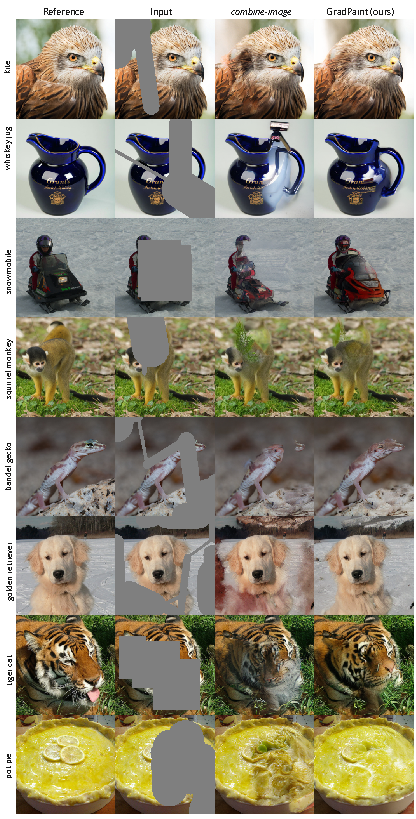
\includegraphics[width=0.8\linewidth]{images/gradpaint/in_latent_samples.pdf} %tried 0.7
  \caption{Qualitative examples from ImageNet with the latent diffusion model. Both the baseline and our algorithm are initialized with the same initial noise map.}
\label{fig:qualitative_latent_imagenet}
\end{figure}


\section{Further Studies}


\subsection{Impact of mask distribution} \label{ood_mask}

Training-free is particularly advantageous since such a method is is agnostic to any 
pre-defined mask distribution to train on, contrary to training-based mehods. We 
illustrate this by comparing our method to LaMa~\citep{lama} on masks outside of 
their pre-defined training distribution. Specifically, we create masks where each 
pixel has a 80\% chance of being masked, masking considerable portions of the image. 
As we can see with Fig.~\ref{fig:ood}, \cite{lama} produces blurry and low-quality
 results while our method produces realistic images. This is further quantitatively 
 validated in Tab.~\ref{abnormal_tab}. 

\begin{figure}[htbp]
  \centering
    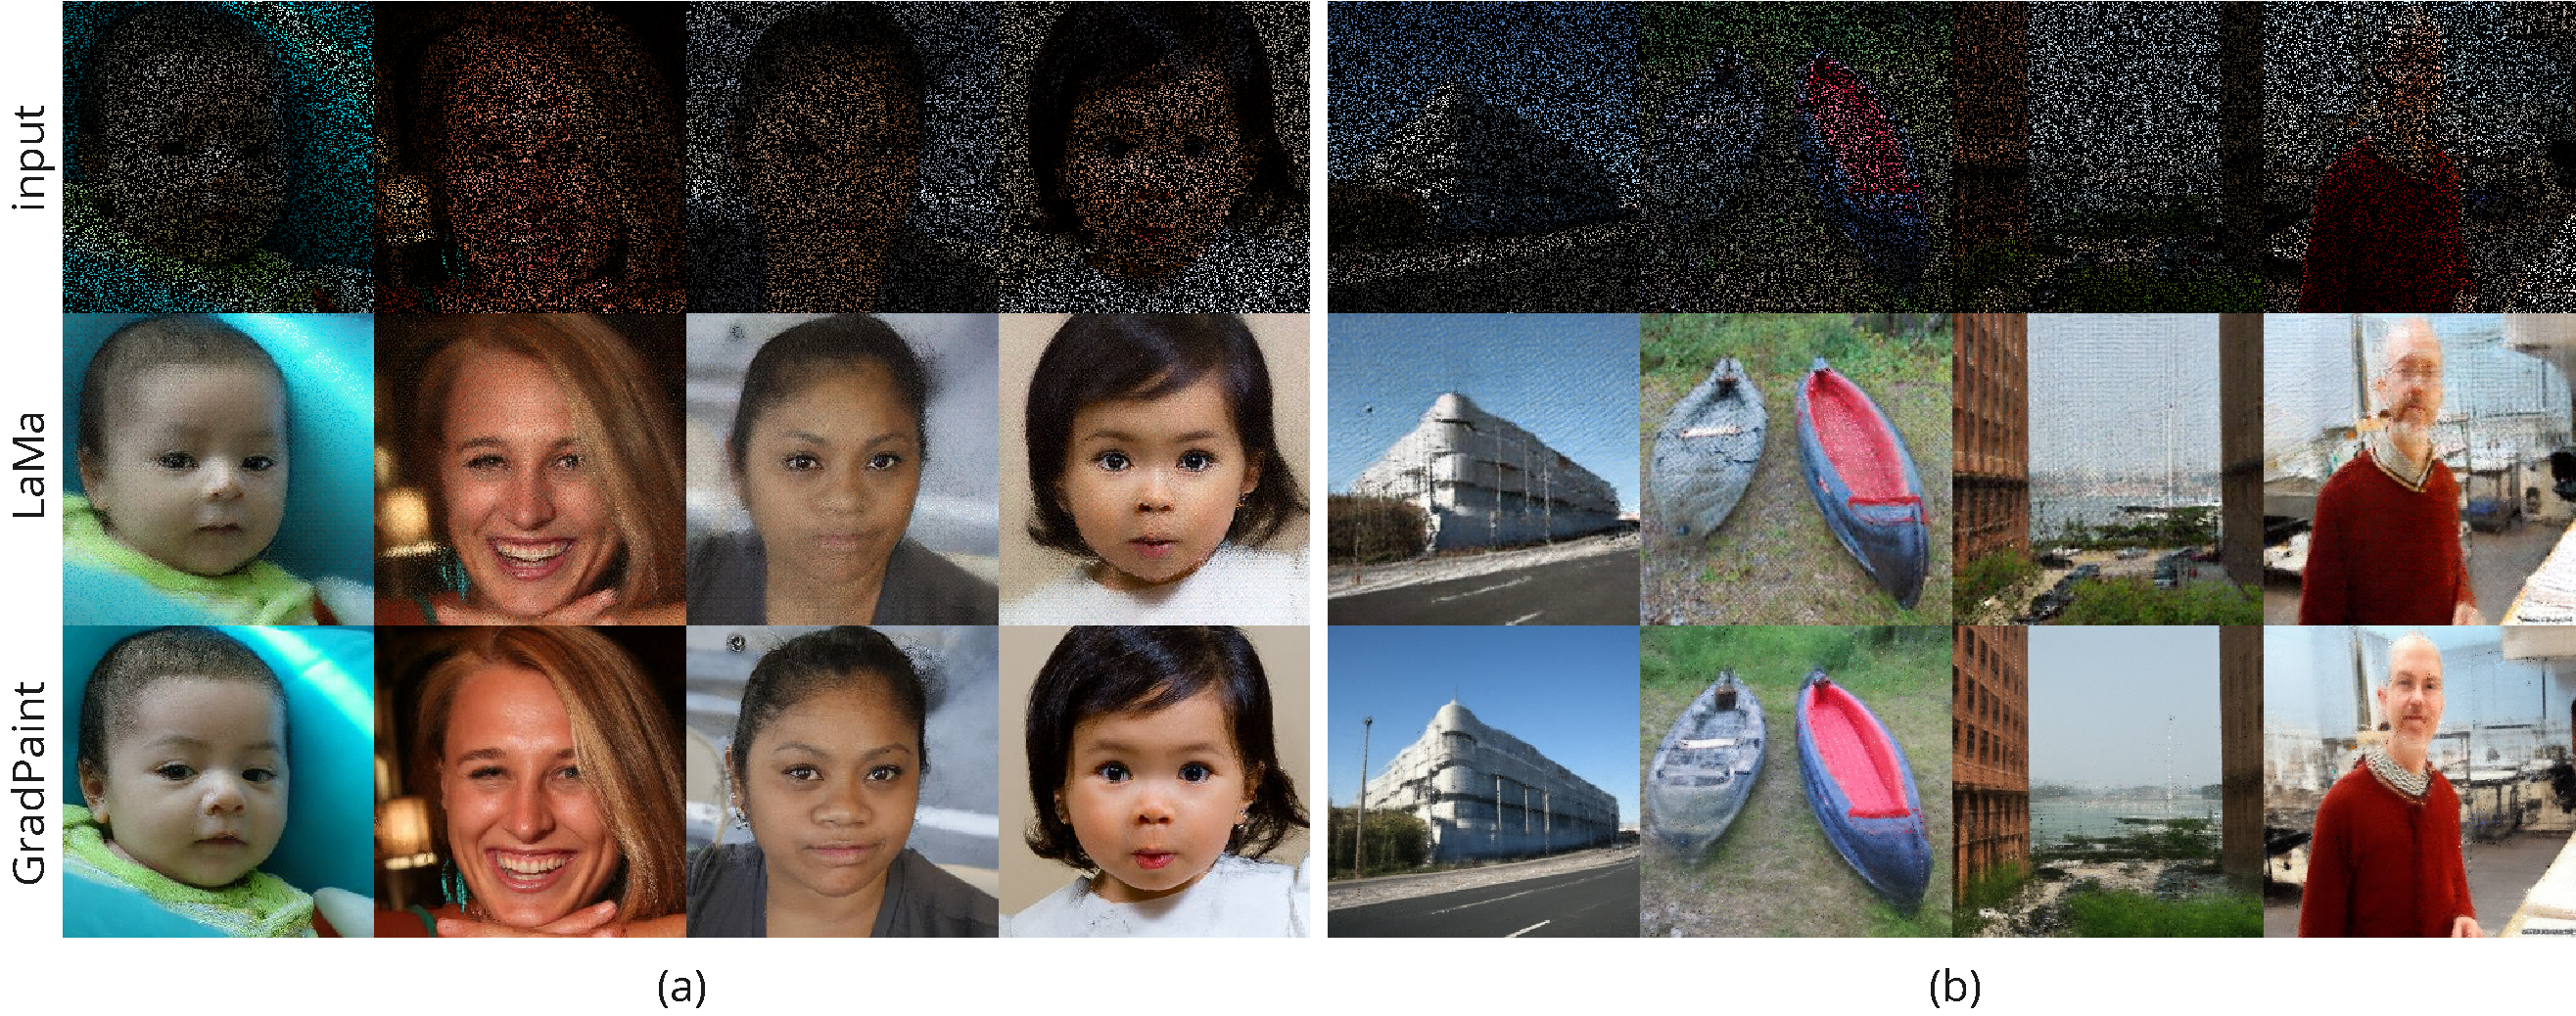
\includegraphics[width=\linewidth]{images/gradpaint/abnormal_masks.pdf}
    \caption{Uncurated results of our method compared to LaMa on out-of-distribution masks. We show images from (a) FFHQ and (b) Places2. LaMa fares poorly on masks outside of the training distribution. Best viewed zoomed and in color.}
    \label{fig:ood}
\end{figure}





\begin{table}[H]
\centering
\begin{tabular}{|l|ll|ll|}
\hline
                   & \multicolumn{2}{c|}{CelebaHQ} & \multicolumn{2}{c|}{Places2} \\ \hline
                   & \multicolumn{1}{l|}{FID$\downarrow$}             & LPIPS$\downarrow$          & \multicolumn{1}{l|}{FID$\downarrow$}            & LPIPS$\downarrow$          \\ \hline
\rowcolor[gray]{0.7}
COPY (oracle)               & \multicolumn{1}{l|}{4.29}           & 0.0          & \multicolumn{1}{l|}{6.47}          & 0.0          \\ \hline

GREYFILL               & \multicolumn{1}{l|}{403.23}           & 1.06          & \multicolumn{1}{l|}{282.01}          & 1.09          \\ \Xhline{4\arrayrulewidth}

LaMa               & \multicolumn{1}{l|}{74.47}           & 0.517          & \multicolumn{1}{l|}{52.63}          & 0.320          \\ \hline

GradPaint & \multicolumn{1}{l|}{\textbf{44.87}}  & \textbf{0.170} & \multicolumn{1}{l|}{\textbf{27.17}} & \textbf{0.277} \\ \hline

\end{tabular}
\caption{Quantitative results comparing our train-free method to a training-based method (LaMa) on CelebaHQ and Places2 using masks outside of LaMa's training distribution.}
\label{abnormal_tab}
\end{table}



\subsection{Inpainting with diversity}


\begin{figure}[htbp]
  \centering
    \includegraphics[width=\linewidth]{images/gradpaint/diversity.pdf}
    \caption{Diversity of select samples from 30 random samples. Images which are well-harmonized are less diverse, e.g. in (1), our method is encouraged to produce a blue background using the small available context, disregarded by the baseline method which produces more diverse but unharmonized backgrounds. Matching columns of samples of (b) and (c) are initialized identically.}
    \label{fig:diversity}
\end{figure}

A method which well-harmonizes an image for the inpainting task will, naturally, produce less diverse images. This can be illustrated in Fig.~\ref{fig:diversity}. Because the baseline method poorly utilizes the surrounding context, samples are diverse but not realistic. On the other hand, our method leverages the surrounding context which produces a more natural result, implying more consistent generations. 
To further analyze the diversity of our samples, we used one single input image and generated 500 outputs, comparing our method with the baseline \emph{combine-image}. We then extracted image features using the inception v3 pre-trained model~\citep{inceptionv3} and display the average of the variance of these features. Tab.~\ref{tab:diversitytab} shows the results. Our method gives diverse samples as the input mask sizes increases, but limits absurd and unharmonized results.

% \begin{figure}[htbp]
%   \centering
%     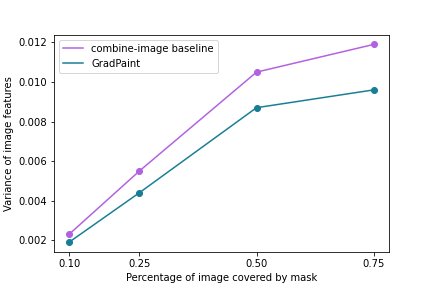
\includegraphics[width=\linewidth]{images/diversitygraph2.png}
%     \caption{Variance of image features for our method (GradPaint) compared to the baseline method, when generating 500 different results for the same input image (and 4 different masks). As we can see, our method expectedly produces more diverse images as the region covered by inpainting mask increases, yet the harmonized results are less diverse than the baseline method.}
%     \label{fig:diversitygraph}
% \end{figure}


\begin{table}[]
\centering
\begin{tabular}{|l|l|l|l|l|}
\hline
\multicolumn{1}{|c|}{ mask coverage (\% of im.)} & \multicolumn{1}{c|}{10\%} & \multicolumn{1}{c|}{25\%} & \multicolumn{1}{c|}{50\%} & \multicolumn{1}{c|}{75\%} \\ \hline
\textit{combine-image}                            & 2.3                       & 5.5                       & 10.5                      & 11.9                      \\ \hline
GradPaint                                         & 1.9                       & 4.4                       & 8.7                       & 9.6                       \\ \hline
\end{tabular}
\caption{Variance of image features (in $10^{-3}$) for GradPaint compared to the baseline method, for 500 generated results using the same input image and increasing-sized masks.  Our method expectedly produces more diverse images as the inpainting mask increases, nearing the diversity of the baseline for large masks.}
\label{tab:diversitytab}
\vspace{-.45cm}
\end{table}





\subsection{Inference Time Study}\label{speed_section}

\begin{figure*}[t!]
    \centering
    \begin{subfigure}[t]{0.5\linewidth}
        \centering
        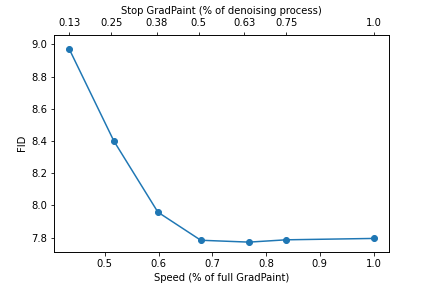
\includegraphics[height=2.3in]{images/gradpaint/speed_fid.png}
        \caption{FID vs. Time tradeoff}
    \end{subfigure}%
    ~ 
    \begin{subfigure}[t]{0.5\linewidth}
        \centering
        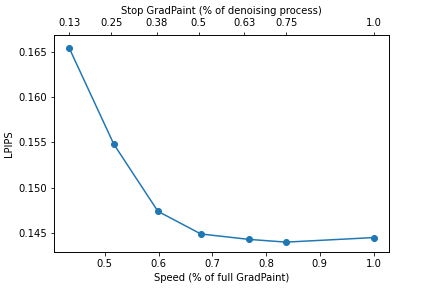
\includegraphics[height=2.3in]{images/gradpaint/speed_lpips.png}
        \caption{LPIPS vs. Time tradeoff}
    \end{subfigure}
    \caption{Performance vs. Time tradeoff, performed on ImageNet. We performed various settings where we early stopped the gradient calculation of GradPaint at $13\%, 25\%, 38\%, 50\%, 63\%, 75\%$ of the denoising process. The most important gains of GradPaint occurs thanks to the early gradient-guidance, and after $63\%$, gradient guiding no longer helps performance. A reasonable early-stopping at $50\%$ of the denoising process reduces the initial time of GradPaint by $33\%$.}
    \label{timsvsacc}
\end{figure*}

Our method requires approximately 3x the compute time of the  gradient-free sampling baselines \emph{combine-image} and 
\emph{combine-noisy}, explained by the added backpropagation of every step of the denoising process. As illustrated in Figure~\ref{fig:intuition}, 
our method succeeds because the prediction $\hat{x}_0$ is aligned and harmonized with the input image early
 on in the diffusion process. We can improve the time of GradPaint by early-stopping the gradient calculation and letting the 
 rest of the denoising process run as in \emph{combine-image}. If the harmonization succeeded well-enough early on, then subsequent
  gradient calculations may not be necessary later in the denoising process, saving valuable compute time. We performed these 
  experiments for various early stopping times of the total denoising process. Fig.~\ref{timsvsacc} shows the performance in terms
   of LPIPS and FID for the various settings. Performing GradPaint after $63\%$ of the denoising process doesn't improve performance, 
   and significantly increases compute time. Stopping the gradient calculation at about $50\%$ of the denoising process achieves the 
   most important gains in performance and allows us to reduce the initial GradPaint time by $33\%$. This early stopping is referred 
   to as "GradPaint-Fast" below.
   
   
Lastly, we compare the inference times of various methods in Table~\ref{tab:comp_times}.
Our method is faster than other diffusion-based methods, even those specifically trained for inpainting (Palette), 
especially when applied to LDMs. We remark that RePaint~\citep{lugmayr2022repaint} takes $313s$ (over 5 minutes!) per image, 
making it unfitting for practical use.


\begin{table}[H]
    \centering
    \begin{tabular}{|l|c|c|c|}
    \hline
    Method           & \multicolumn{1}{l|}{Training-Free?} & Diffusion-based? & Inference time per image (s)  \\ \hline
    LaMa             & \multicolumn{1}{l|}{} &               & 0.02                                                                          \\ \hline
    Palette          & \multicolumn{1}{l|}{} & \checkmark              & 56                                                                            \\ \hline
    RePaint          & \checkmark  & \checkmark                                 & 313                                                                           \\ \hline
    MCG              & \checkmark   & \checkmark                                & 52                                                                            \\ \hline
    GradPaint        & \checkmark  & \checkmark                                 & 66                                                                            \\ \hline
    GradPaint-Fast   & \checkmark  & \checkmark                                 & 44                                                                          \\ \hline
    GradPaint-Latent & \checkmark & \checkmark                                  & 7.2                                                                           \\ \hline
    \end{tabular}
\caption{Inference times for various methods. As we can see, our method is faster than other diffusion-based methods, especially when applied to Latent Diffusion Models}
\label{tab:comp_times}
\end{table}\textbf{}



\section{Conclusion}

We have presented GradPaint, a training-free algorithm that guides the generative process of diffusion to better perform 
inpainting operations when given real images. GradPaint improves upon baselines by better harmonizing generated content 
inside the inpainting mask with known regions of the input image, which is done via gradient descent computed from a 
dedicated harmonization loss. Extensive qualitative and quantitative experiments demonstrate the superiority of our method, 
which is able to outperform methods trained specifically for inpainting.

It is important to note that many open-source diffusion models are trained with large amounts of web-scraped data, thus 
inheriting their biases. Applying our method onto these models could potentially reinforce harmful cultural biases. We 
believe open-sourcing editing algorithms in a research context contributes to a better understanding of these biases and 
will aid the community to mitigate them in the future.

In our quest to perform real-image editing, our method GradPaint achieves perfect fidelity to the input image in regions outside 
of the mask and well-edited images thanks to our harmonization guidance. Our method benefits from an easy inversion scheme of 
iteratively denoising the input image (which avoids the drawbacks of Chapter~\ref{chapter:magec}) and benefits from a powerful generative 
prior (which avoids the drawbacks of Chapter~\ref{chapter:flexit}). Our method can generalize well to many types of masks, 
unlike fully-supervised methods which perform poorly with masks outside of the training distribution. 
It's important to note, however, that GradPaint's editing scheme is still limited, mainly to object removal or addition. For example, 
if we wish to change a person's facial 
expression, changes would be required all across the face (eye expression, mouth shape, modified wrinkles, eyebrows lifted, etc.). 
Our strategy would thus not assure coherence to the input image with such a large mask. Nontheless,
our method exploits the generative power of today's ever-growing generative models to effectively and realistically 
perform aeasthetic image inpainting.